\documentclass[a4paper,twoside]{article}
\usepackage[T1]{fontenc}
\usepackage[bahasa]{babel}
\usepackage{graphicx}
\usepackage{graphics}
\usepackage{float}
\usepackage[cm]{fullpage}
\pagestyle{myheadings}
\usepackage{etoolbox}
\usepackage{setspace} 
\usepackage{lipsum} 
\usepackage{enumitem}
\usepackage{listings}
\setlength{\headsep}{30pt}
\usepackage[inner=2cm,outer=2.5cm,top=2.5cm,bottom=2cm]{geometry} %margin
% \pagestyle{empty}

% ############################################################################
% Library tambahan
\usepackage{graphicx}
\usepackage{subcaption}
\usepackage{enumitem}
\usepackage{multirow}
\usepackage[table,xcdraw]{xcolor}
% Beamer presentation requires \usepackage{colortbl} instead of
\usepackage[table,xcdraw]{xcolor}
\usepackage{hyperref}
\definecolor{biruFtis}{RGB}{0,166,226}
\hypersetup{
    colorlinks=true,
    % Menggunakan format rgb
    linkcolor= red,
    filecolor= biruFtis,
    urlcolor= biruFtis,
    pdftitle={Overleaf Example},
    pdfpagemode=FullScreen,
    }

\usepackage{listings}
\renewcommand{\lstlistingname}{Kode}
\usepackage{xcolor}
% Definisikan bahasa JavaScript untuk mendukung ReactJS
\lstdefinelanguage{JavaScript}{
    keywords={break, case, catch, continue, debugger, default, delete, do, else, finally, for, function, if, in, instanceof, new, return, switch, this, throw, try, typeof, var, void, while, with, let, const, await, async, import, from, export, default},
    morekeywords={useState, useEffect, useContext, useReducer, className, render, component, React},
    sensitive=true,
    comment=[l]//,
    commentstyle=\color{green!50!black}\itshape,
    stringstyle=\color{red},
    morestring=[b]',
    morestring=[b]",
}
%listing khusus untuk penulisan kode program, menggunakan font Bera Mono
\lstset{numbers=left,stepnumber=1, numbersep=5pt, frame=single,frameround={tttt},
	tabsize=4, breaklines=true, basicstyle=\fontfamily{fvm}\selectfont\tiny, 
	commentstyle=\itshape\color{gray}, keywordstyle=\bfseries\color{blue}, 
	identifierstyle=\color{black}, stringstyle=\color{orange},
	literate={-}{-}1{-\,-}{--}1
} 
% END LIBARY TAMBAHAN

\setlength{\headsep}{30pt}
\usepackage[inner=2cm,outer=2.5cm,top=2.5cm,bottom=2cm]{geometry} %margin
% \pagestyle{empty}
% ############################################################################

\usepackage{array}
\usepackage{tabularx}
\renewcommand{\arraystretch}{1.5} % Mengatur jarak antar baris



\makeatletter
\renewcommand{\@maketitle} {\begin{center} {\LARGE \textbf{ \textsc{\@title}} \par} \bigskip {\large \textbf{\textsc{\@author}} }\end{center} }
\renewcommand{\thispagestyle}[1]{}
\markright{\textbf{\textsc{Laporan Perkembangan Pengerjaan Tugas Akhir\textemdash Sem. Ganjil 2024/2025}}}

\onehalfspacing
 
\begin{document}

\title{\@judultopik}
\author{\nama \textendash \@npm} 

%ISILAH DATA BERIKUT INI:
\newcommand{\nama}{Ade Rimbo Spencher}
\newcommand{\@npm}{6182001060}
\newcommand{\tanggal}{16/12/2024} %Tanggal pembuatan dokumen
\newcommand{\@judultopik}{Pengembangan Generator Konten Website berbasis Application Programming Interface (API) untuk Mendukung Interoperabilitas yang Aman dan Andal} % Judul/topik anda
\newcommand{\kodetopik}{GDK5704ACS}
\newcommand{\jumpemb}{1} % Jumlah pembimbing, 1 atau 2
\newcommand{\pembA}{Dr. Gede Karya, S.T., S.E., M.T., CISA}
\newcommand{\pembB}{-}
\newcommand{\semesterPertama}{57 - Ganjil 24/25} % semester pertama kali topik diambil, angka 1 dimulai dari sem Ganjil 96/97
\newcommand{\lamaSkripsi}{1} % Jumlah semester untuk mengerjakan tugas akhir s.d. dokumen ini dibuat
\newcommand{\kulPertama}{Tugas Akhir 1} % Kuliah dimana topik ini diambil pertama kali
\newcommand{\tipePR}{B} % tipe progress report :
% A : dokumen pendukung untuk pengambilan ke-2 di Tugas Akhir 1
% B : dokumen untuk reviewer pada presentasi dan review Tugas Akhir 1
% C : dokumen pendukung untuk pengambilan ke-2 di Tugas Akhir 2

% Dokumen hasil template ini harus dicetak bolak-balik !!!!

\maketitle

\pagenumbering{arabic}

% \section{Data Tugas Akhir}
% Pembimbing utama/tunggal: {\bf \pembA}\\
Pembimbing pendamping: {\bf \pembB}\\
Kode Topik : {\bf \kodetopik}\\
Topik ini sudah dikerjakan selama : {\bf \lamaSkripsi} semester\\
Pengambilan pertama kali topik ini pada : Semester {\bf \semesterPertama} \\
Pengambilan pertama kali topik ini di kuliah : {\bf \kulPertama} \\
Tipe Laporan : {\bf \tipePR} -
\ifdefstring{\tipePR}{A}{
			Dokumen pendukung untuk {\BF pengambilan ke-2 di Tugas Akhir 1} }
		{
		\ifdefstring{\tipePR}{B} {
				Dokumen untuk reviewer pada presentasi dan {\bf review Tugas Akhir 1}}
			{	Dokumen pendukung untuk {\bf pengambilan ke-2 di Tugas Akhir 2}}
		}
        
% \section{Latar Belakang}
% Dalam pengembangan aplikasi berbasis \textit{website}, \textit{website} tidak hanya dituntut untuk memiliki tampilan yang informatif dan interaktif, tetapi juga memerlukan standar keamanan serta keandalan. Aplikasi yang terhubung langsung ke internet rentan terhadap berbagai ancaman siber, seperti pencurian data sensitif maupun manipulasi sistem, yang pada akhirnya dapat mengganggu operasional bisnis. Bagi suatu organisasi, risiko ini meningkat ketika data internal yang sifatnya sensitif harus diakses oleh aplikasi \textit{website} yang bersifat publik.

Salah satu pendekatan untuk mengurangi risiko tersebut adalah dengan memisahkan komponen publik dari lingkungan internal organisasi. Melalui pengaturan ini, aplikasi \textit{website} dapat difungsikan sebagai antarmuka publik yang menampilkan data dan konten, sedangkan aplikasi internal yang menyimpan logika bisnis dan data sensitif tetap berada pada lingkungan yang lebih terbatas. Langkah ini mengurangi akses eksternal langsung ke sumber data internal, sehingga memperkuat lapisan keamanan dan mengurangi paparan terhadap ancaman siber.

Meskipun demikian, tantangan lain muncul ketika sebuah organisasi memiliki beragam aplikasi internal yang menyuplai data ke aplikasi \textit{website}. Kondisi ini sering menimbulkan kompleksitas dalam integrasi data, pengelolaan konten, serta sinkronisasi informasi, karena masing-masing aplikasi internal dapat memiliki skema data, format, atau aturan bisnis yang berbeda. Tanpa mekanisme integrasi yang terpusat, menjaga konsistensi konten antara aplikasi internal dan aplikasi \textit{website} menjadi sulit, sehingga berdampak pada kualitas informasi yang disajikan kepada pengguna.

Untuk mengatasi tantangan tersebut, dalam tugas akhir ini dikembangkan sebuah \textit{generator} konten \textit{website} berbasis API yang dirancang dengan fokus pada keamanan serta keandalan. Sistem ini tidak hanya mengandalkan templat statis, tetapi juga memanfaatkan data aplikasi web dan data yang diambil secara terkini dari aplikasi internal. Dengan demikian, proses \textit{generate content website} selalu mengacu pada data paling mutakhir, sekaligus memastikan data sensitif tidak terekspos secara langsung. Dari sisi keandalan, sistem mengimplementasikan mekanisme sinkronisasi yang berlangsung dalam dua tahap:  
(1) Sinkronisasi data dari aplikasi internal ke aplikasi\textit{website} dilakukan pada saat proses \textit{generate website}, sehingga konten pada \textit{website} menggunakan data paling mutahir.
(2) Sinkronisasi data dari \textit{website} ke aplikasi internal dilakukan secara terjadwal, di mana data yang akan disinkronkan, terlebih dahulu diverifikasi berdasarkan templat dan aturan yang tersimpan pada basis data.

Dengan pendekatan ini, organisasi dapat membangun aplikasi \textit{website} yang aman dan handal tanpa mengorbankan perlindungan data internal. Seluruh proses integrasi dan sinkronisasi dikelola secara terkontrol melalui API \textit{generator} konten \textit{website}.

Secara umum, alur kerja sistem ini dapat dilihat pada Gambar \ref{fig:GambaranUmum}. Prosesnya mencakup tiga langkah utama:
\begin{enumerate}
    
    \item \textbf{Pembangunan aplikasi \textit{website}:} \textit{Generator} (G) membangun aplikasi \textit{website} (AW) berdasarkan templat yang tersimpan di Basis Data Templat (T), data aplikasi \textit{website} yang sudah ada aplikasi internal (AI), serta data asli aplikasi internal (AI) yang terkini.
    
    \item \textbf{Sinkronisasi data terjadwal:} \textit{Sinkronisator} (S) secara berkala mengambil data dari aplikasi \textit{website} (AW), memvalidasinya berdasarkan aturan yang ada di basis data templat (T), lalu mengirimkannya kembali ke aplikasi internal (AI).
    
    \item \textbf{Akses aman oleh pengguna:} Pengguna mengakses aplikasi \textit{website} (AW) melalui mekanisme \textit{Single Sign-On} (SSO) demi menjaga keamanan akses.
    
\end{enumerate}

\begin{figure}[H]
    \centering
    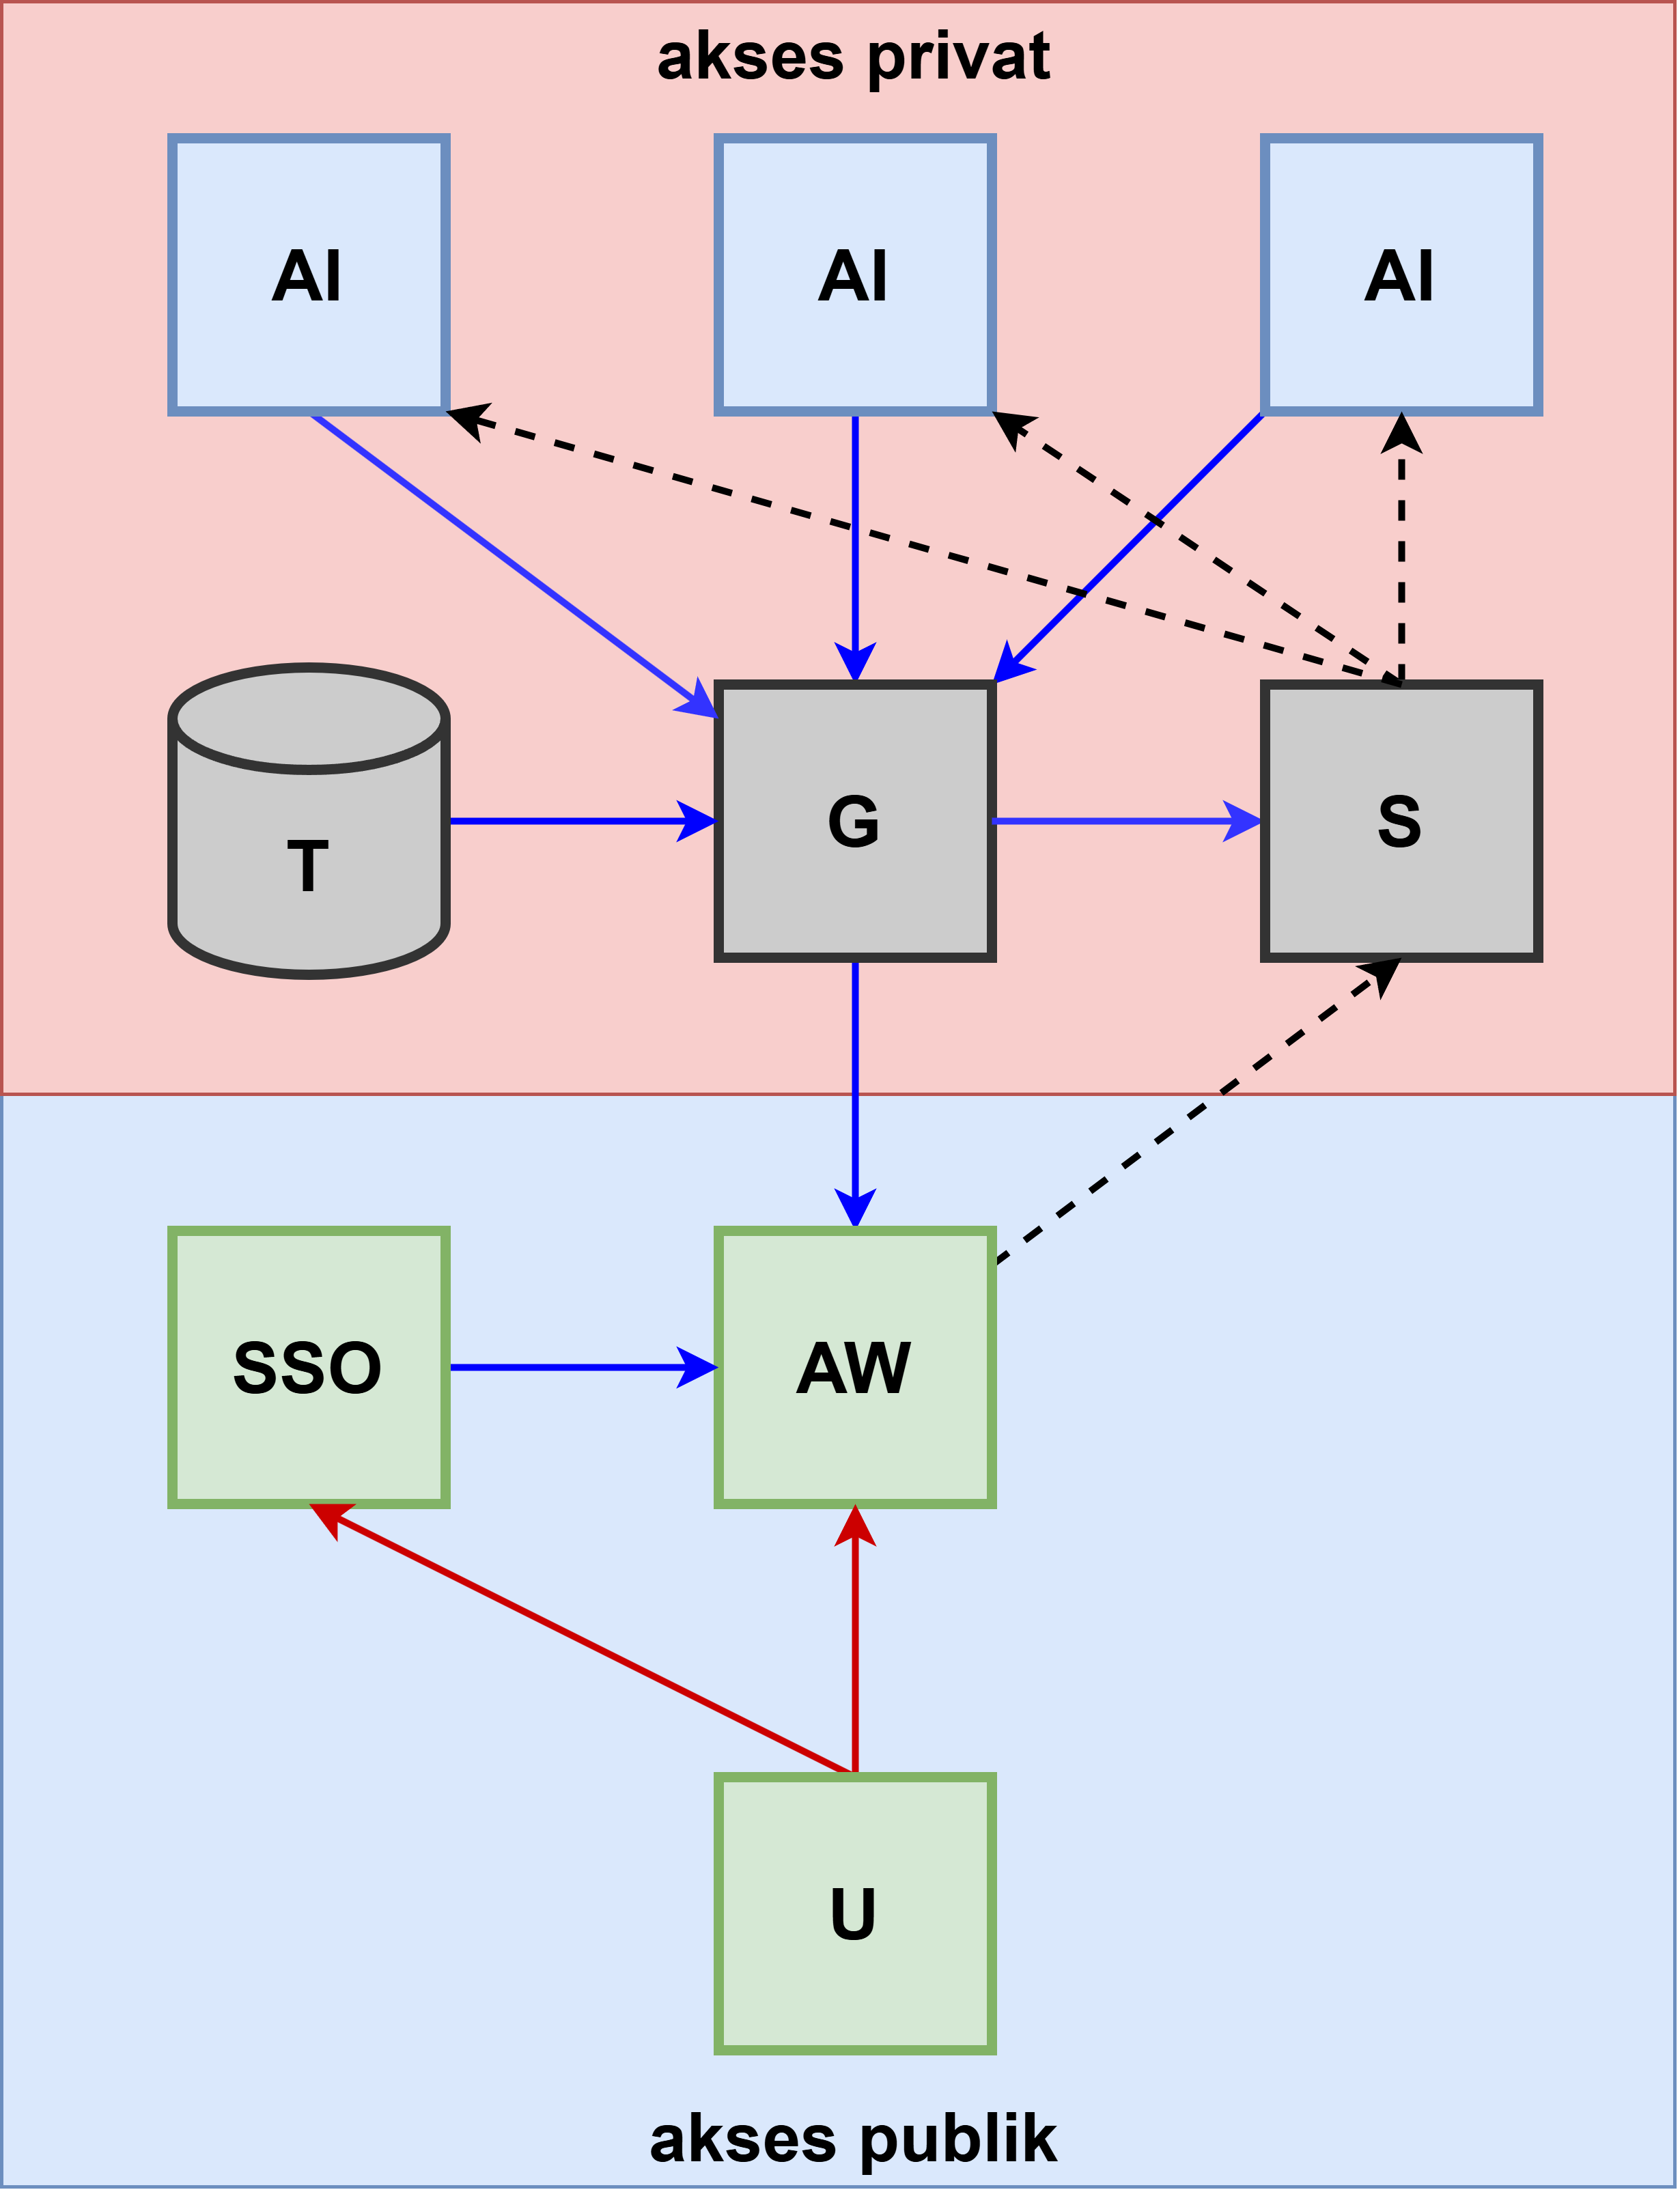
\includegraphics[width=0.5\linewidth]{figures/GambaranUmum.png}
    \caption{Gambaran Umum Arsitektur Sistem}
    \label{fig:GambaranUmum}
\end{figure}


% \section{Rumusan Masalah}
% \begin{enumerate}
    \item Fitur-fitur apa saja yang harus dimiliki oleh generator konten website berbasis API?
    
    \item Bagaimana merancang generator konten website berbasis API yang aman dan handal?
    
    \item Bagaimana mengimplementasikan generator konten website berbasis API dan contoh aplikasi internal sebagai sumber data templat?
    
    \item Bagaimana menguji generator konten website berbasis API dalam menghasilkan minimal tiga website?
    
\end{enumerate}

% \section{Tujuan}
% \begin{enumerate}
    
    \item Mengidentifikasi fitur-fitur yang akan diterapkan generator konten website berbasis API.
 
    \item Merancang generator konten website berbasis API yang aman dan handal.

    \item Mengimplementasikan generator konten berbasis API dan contoh aplikasi internal sebagai sumber data templat.

    \item Menguji generator konten website berbasis API dalam menghasilkan minimal tiga website.
    
\end{enumerate}

\section{Detail Perkembangan Pengerjaan Tugas Akhir}
Detail bagian pekerjaan tugas akhir sesuai dengan rencana kerja/laporan perkembangan terakhir :

\begin{enumerate}
    
    \item \textbf{Melakukan studi literatur mengenai pengembangan aplikasi berbasis web}\\
    {\bf Status :} Ada sejak rencana kerja tugas akhir.\\
    {\bf Hasil :}\\
    Berdasarkan hasil studi literatur yang sudah dilakukan dari sumber sebagai berikut :
    \begin{itemize}
        \item WWW: past, present, and future
        \item What Is a Web Application? Web Application Design Handbook
        \item Effective Java Programming Language Guide
        \item PHP and MySQL Web Development
        \item The Go Programming Language
        \item Automate the Boring Stuff with Python: Practical Programming for Total Beginners
        \item Enterprise Application Integration: A Wiley Tech Brief
        \item Designing Web APIs: Building APIs That Developers Love
        \item OAuth 2 in Action
    \end{itemize}
Didapatkan hasil berikut ini :
\begin{enumerate}[label*=\arabic*.,ref=\arabic*]
    \item Konsep Dasar\\
        Web, atau yang secara formal dikenal sebagai \textit{World Wide Web} (WWW) didefinisikan sebagai semesta informasi yang dapat diakses melalui jaringan global. WWW sebagian besar dihuni oleh teks, gambar, dan animasi yang saling terkait, dengan sesekali menampilkan suara, video, dan dunia tiga dimensi. Web dirancang sebagai sebuah ruang di mana orang dapat berkolaborasi dalam sebuah proyek.
        
        Aplikasi memiliki fokus pada interaksi pengguna untuk menyelesaikan tugas tertentu. Aplikasi ini dapat berupa sistem manajemen data, alat analisis, atau platform kolaborasi. Aplikasi ini dirancang untuk memberikan pengalaman yang efisien dan sering kali dilengkapi dengan fitur seperti keamanan, manajemen sesi, dan integrasi dengan sistem lain.

        Aplikasi berbasis web dirancang untuk lebih dari sekedar menyediakan informasi seperti halaman web. Memungkinkan pengguna untuk melakukan input data, bertransaksi, atau mengakses layanan tertentu secara \textit{online}. Aplikasi berbasis web biasanya membutuhkan interaksi berkelanjutan antara pengguna dan server untuk menyimpan atau memproses data. Aplikasi berbasis web dirancang untuk mendukung berbagai kebutuhan bisnis, mulai dari sistem manajemen internal hingga \textit{platform e-commerce}.
        
    \item Komponen dan Teknologi\\
        Aplikasi berbasis web terdiri dari berbagai komponen yang bekerja sama untuk memberikan fungsionalitas dan pengalaman yang optimal kepada pengguna. Setiap komponen memiliki tanggung jawab tertentu, mulai dari antarmuka pengguna hingga pengolahan data di \textit{back-end}.

        % Jelaskan apa itu framework dan library disini

        Berikut adalah komponen dan teknologi pada aplikasi berbasis web:

        \begin{enumerate}[label=\alph*.]
            \item Front-End (Client-Side)\\
                \textit{Front-end} adalah bagian aplikasi yang langsung berinteraksi dengan pengguna. Ini mencakup semua elemen visual dan antarmuka pengguna yang dapat dilihat dan digunakan oleh pengguna.

                Teknologi yang digunakan:
                \begin{itemize}
                    \item HTML\\
                        \textit{HyperText Markup Language} (HTML) adalah bahasa \textit{markup} standar untuk membuat dan menyusun halaman web serta aplikasi web. Elemen-elemen HTML memungkinkan pengembang untuk menentukan berbagai komponen dalam sebuah halaman, seperti teks, gambar, tabel, dan formulir. Dalam konteks aplikasi berbasis web, HTML sering menjadi fondasi untuk menampilkan antarmuka pengguna yang kemudian diperluas dengan CSS dan JavaScript. 
                    \item CSS\\
                        \textit{Cascading Style Sheet} (CSS) bertanggung jawab atas tampilan dan nuansa visual halaman web. Ini memungkinkan pengembang untuk menerapkan gaya seragam untuk elemen yang ditulis dalam HTML, mengatur tata letak, warna, tulisan, dan aspek visual lainnya. Dalam aplikasi web, CSS memungkinkan antarmuka menjadi lebih menarik dan responsif terhadap berbagai perangkat, termasuk komputer desktop dan perangkat seluler. 
                    \item JavaScript\\
                        JavaScript adalah bahasa pemrograman yang digunakan untuk membuat halaman web menjadi interaktif. Berbeda dengan HTML yang statis dan CSS yang fokus pada presentasi, JavaScript memungkinkan implementasi fitur-fitur dinamis pada halaman web yang dapat berinteraksi dengan pengguna, mengendalikan \textit{browser}, dan secara dinamis mengubah dokumen yang telah ditampilkan. Misalnya, JavaScript dapat digunakan untuk menambahkan animasi, memuat konten baru tanpa harus memuat ulang halaman, mengambil data dari server secara asinkron (AJAX), dan mengolah formulir. JavaScript juga sangat penting dalam pengembangan \textit{single-page application} (SPA), di mana pengguna dapat menikmati pengalaman web yang mulus tanpa pemuatan halaman yang terputus-putus.
                \end{itemize}

                Contoh penggunakan HTML, CSS, dan JavaScript secara bersamaan:
                \begin{lstlisting}[language=Javascript,caption={HTML, CSS dan JavaScript}]
<!DOCTYPE html>
<html lang="en">
<head>
    <meta charset="UTF-8">
    <meta name="viewport" content="width=device-width, initial-scale=1.0">
    <title>Contoh Sederhana</title>
    <style>
        /* Menggabungkan CSS langsung di dalam tag <style> */
        body {
            font-family: Arial, sans-serif;
            padding: 20px;
            text-align: center;
        }

        p {
            color: #333;
        }

        button {
            padding: 10px 20px;
            font-size: 16px;
            cursor: pointer;
            background-color: #4CAF50;
            color: white;
            border: none;
            border-radius: 5px;
        }
    </style>
</head>
<body>
    <p id="message">Halo, ini adalah contoh penggunaan HTML, CSS, dan JavaScript!</p>
    <button onclick="changeColor()">Ubah Warna</button>

    <script>
        // Menggabungkan JavaScript langsung di dalam tag <script>
        function changeColor() {
            document.getElementById("message").style.color = "blue";
        }
    </script>
</body>
</html>
\end{lstlisting}
                
                Selain menggunakan HTML, CSS dan JavaScript, pengembangan \textit{client-side} juga dapat menggunakan \textit{framework} seperti React dan Angular.
                
            \item Back-End (Server-Side)\\
                \textit{Back-end} adalah komponen yang berperan untuk menangani logika bisnis aplikasi dan proses di balik layar yang tidak terlihat oleh pengguna.

                Teknologi yang digunakan berdasarkan bahasa pemrograman sebagai berikut:
                \begin{itemize}
                    \item JavaScript\\
                        JavaScript secara tradisional digunakan di sisi klien untuk membuat halaman web interaktif, tetapi dengan hadirnya Node.js, penggunaannya kini meluas ke sisi server. Node.js adalah \textit{runtime} JavaScript berbasis V8 (engine JavaScript Google Chrome) yang memungkinkan eksekusi kode secara cepat di luar \textit{browser}. Dirancang untuk membangun aplikasi jaringan yang skalabel, Node.js menggunakan model \textit{non-blocking I/O} dan asinkronus.

                        Express.js, sebagai \textit{framework} untuk Node.js, mempermudah pengelolaan rute, permintaan, dan tanggapan dalam aplikasi web. Dengan pendekatan minimalis, Express.js memungkinkan pengaturan \textit{middleware} dan pengelolaan HTTP tanpa banyak abstraksi tambahan, mendukung pengembang dalam membangun aplikasi secara lebih fleksibel.
                    \item Java\\
                        % Penjelasan tentang Java sebagai server-side, spring boot
                        Java merupakan sebuah bahasa pemrograman yang fleksibel dan produktif, dengan fokus pada kualitas kode. Java dapat digunakan untuk membangun komponen perangkat lunak yang dapat digunakan kembali melalui pendekatan API. Di dalam Java, terdapat Spring Boot yang mendukung pengaturan otomatis, manajemen dependensi, dan integrasi dengan berbagai pustaka serta layanan. Spring Boot dirancang untuk mempermudah pengembangan aplikasi berskala besar dengan pendekatan minimal konfigurasi. 
                    \item PHP\\
                        % Penjelasan tentang PHP sebagai server-side, laravel
                        PHP merupakan sebuah bahasa pemrograman sisi server yang dirancang khusus untuk pengembangan web. PHP memungkinkan integrasi kode dalam halaman HTML untuk menghasilkan konten dinamis. Kini merupakan salah satu bahasa pemrograman terpopuler di dunia, terutama karena kemudahan penggunaannya, kinerja tingga, dan sifatnya yang \textit{open source}. Sebagai salah satu contoh \textit{framework} PHP yang paling populer yaitu Laravel. Laravel dirancang untuk mempermudah pengembangan aplikasi web dengan menyediakan fitur seperti routing, \textit{middleware}, serta alat untuk pengelolaan database dan autentikasi. 
                    \item Go\\
                        % Penjelasan tentang Go sebagai server-side dan frameworknya
                        Go merupakan sebuah bahasa pemrograman yang andal dan dirancang untuk membangun perangkat lunak modern, terutama di sisi server. Go menonjol karena fitur-fitur seperti pengelolaan memori otomatis, sistem tipe yang sederhana, serta kemampuan bawaan untuk pemrograman konkuren. Salah satu \textit{framework} populer dalam ekosistem Go adalah Gin. Gin mendukung pengembangan aplikasi web dengan pendekatan minimalis dan performa tinggi. Gin mempermudah pengelolaan routing, \textit{middleware}, serta pengelolaan permintaan HTTP dengan API yang sederhana namun fleksibel. 
                    \item Python\\
                        % Penjelasan tentang Python sebagai server-side dan frameworknya
                        Python didefinisikan sebagai bahasa pemrograman serbaguna yang mudah dipelajari dan digunakan. Python terkenal dengan sintaksisnya yang sederhana dan pustaka yang kaya, menjadikannya pilihan utama untuk berbagai aplikasi, termasuk pemrograman server-side, otomatisasi tugas, analisis data, dan pengembangan web.
                        \textit{Framework} populer untuk pengembangan web menggunakan Python adalah Django dan Flask. Django adalah\textit{ framework} berbasis Python yang bersifat penuh fitur (full-stack), mendukung skalabilitas, keamanan, dan efisiensi untuk aplikasi web besar. Flask, di sisi lain, lebih minimalis, cocok untuk proyek yang membutuhkan fleksibilitas tinggi dan kontrol penuh atas struktur aplikasi.
                \end{itemize}
            
            \item Basis Data\\
                Basis data bertugas untuk menyimpan dan mengelola data aplikasi secara sistematis agar dapat diakses dengan cepat dan aman.
                
                Teknologi yang digunakan:
                \begin{itemize}
                    \item SQL\\
                        % Penjelasan tentang SQL dan contoh databasenya (Mysql, PostgreSQL)
                        SQL merupakan sebuah \textit{Structured Query Language}, yaitu bahasa standar untuk mengakses dan mengelola sistem manajemen basis data relasional (RDBMS). 
                        MySQL merupakan salah satu basis data yang digunakan untuk menyimpan data. MySQL adalah sistem manajemen basis data relasional (RDBMS) yang cepat, andal, dan mendukung banyak pengguna secara bersamaan. PostgreSQL merupakan sistem manajemen basis data relasional \textit{open-source} yang dikenal karena mendukung standar SQL dan menyediakan banyak fitur yang biasanya ditemukan dalam sistem basis data komersial. PostgreSQL sering digunakan dalam aplikasi web yang membutuhkan skalabilitas dan integritas data yang tinggi.
                    \item \textit{NoSQL}\\
                        % Penjelasan tentang NoSQL dan contoh databasenya (MongoDB)
                        \textit{NoSQL} merujuk pada basis data non-relasional yang dirancang untuk menangani data besar dengan struktur fleksibel seperti dokumen, graf, atau key-value store. MongoDB adalah salah satu sistem basis data \textit{NoSQL} yang paling populer. Penggunaan MongoDB memudahkan pengembang untuk menyimpan dan mengambil data dengan struktur yang fleksibel dan menjadikannya ideal untuk aplikasi yang berkembang cepat. 
                \end{itemize}
                
        \end{enumerate}

    \item Arsitektur\\
        Arsitektur Aplikasi Berbasis Web menggambarkan cara komponen \textit{front-end}, \textit{back-end}, dan basis data yang saling berinteraksi untuk memberikan layanan kepada pengguna. Pemilihan arsitektur sangat bergantung pada kebutuhan aplikasi, skala, kompleksitas, dan sumber daya yang tersedia. Setiap jenis arsitektur memiliki keunggulan dan kekurangan, sehingga perlu dipilih sesuai dengan tujuan aplikasi yang akan dikembangkan. Berikut adalah beberapa jenis arsitektur pada aplikasi berbasis web:

        \begin{enumerate}[label=\alph*.]
            \item Monolithic Architecture\\
                Arsitektur ini menyusun aplikasi sebagai satu kesatuan yang terintegrasi penuh, di mana semua komponen termasuk antarmuka pengguna, logika bisnis, dan akses data berada dalam satu unit aplikasi.
                
            \item Microservice Architecture\\
                Dalam arsitektur ini, aplikasi dipecah menjadi layanan-layanan kecil yang independen, di mana setiap layanan bertanggung jawab atas fungsi tertentu dan berkomunikasi melalui API.
            
            \item Serverless Architecture\\
                Serverless architecture adalah pendekatan di mana pengembang tidak perlu mengelola server secara langsung. Aplikasi dijalankan pada infrastruktur \textit{cloud}, dan sumber daya diberikan secara otomatis berdasarkan permintaan.
            
            \item Three-Tier Architecture\\
                Arsitektur ini memisahkan aplikasi menjadi tiga lapisan utama:

                \begin{itemize}
                    \item Lapisan Presentasi (Presentation Layer): Menangani antarmuka pengguna (frontend).
                    \item Lapisan Logika Bisnis (Business Logic Layer): Mengelola aturan dan proses aplikasi.
                    \item Lapisan Data (Data Layer): Berisi dan mengelola data aplikasi.
                \end{itemize}
        \end{enumerate}
        
    \item Pendekatan Pengembangan\\
        Pendekatan pengembangan aplikasi web merujuk pada metode atau teknik yang digunakan untuk merender halaman web dan menyajikannya kepada pengguna. Pilihan pendekatan sangat bergantung pada kebutuhan aplikasi, performa yang diinginkan, dan pengalaman pengguna yang diharapkan.
        \begin{enumerate}[label=\alph*.]
            \item Server-Side Rendering (SSR)\\
                Server-Side Rendering (SSR) adalah pendekatan di mana halaman web diproses sepenuhnya di server, kemudian dikirimkan kepada \textit{browser} dalam bentuk HTML yang sudah siap ditampilkan.
                
            \item Client-Side Rendering (CSR)\\
                Client-Side Rendering (CSR) adalah pendekatan di mana halaman web di render di sisi \textit{browser} menggunakan JavaScript. Server hanya mengirimkan dokumen HTML kosong dan JavaScript yang diperlukan untuk membangun halaman.
            
            \item Static Site Generation (SSG)\\
                Static Site Generation (SSG) adalah pendekatan dimana halaman web dihasilkan secara statis selama proses build dan disajikan langsung dari server atau CDN. Halaman ini tidak berubah kecuali dilakukan rebuild.
                
            \item Progressive Web Apps (PWA)\\
                Progressive Web Apps (PWA) adalah aplikasi web yang dirancang untuk memberikan pengalaman pengguna yang mirip dengan aplikasi native di perangkat mobile, tetapi tetap menggunakan teknologi web. PWA memanfaatkan fitur \textit{browser} modern untuk bekerja secara offline, memberikan notifikasi, dan memiliki akses ke perangkat keras.
                
        \end{enumerate}
\end{enumerate} 
    
    \item \textbf{Melakukan studi literatur mengenai \textit{Enterprise Application Integration} (EAI)}\\
    {\bf Status :} Ada sejak rencana kerja tugas akhir.\\
    {\bf Hasil :}\\
    Berdasarkan hasil studi literatur, berikut hal yang didapatkan :
\begin{enumerate}[label*=\arabic*.,ref=\arabic*]
    \item Konsep Dasar \\
    \textit{Enterprise Application Integration} (EAI) sebuah teknologi yang bertujuan untuk menghubungkan berbagai aplikasi yang digunakan dalam suatu organisasi atau perusahaan, sehingga informasi dapat dipertukarkan secara lancar. EAI memiliki beberapa tujuan yaitu untuk sinkronisasi data, otomasi proses bisnis dan fleksibilitas sistem. Beberapa elemen utama di dalam EAI adalah \textit{middleware}, adaptor, dan model data yang terintegrasi. Salah satu keuntungan penggunaan EAI adalah pengurangan redundansi data, di mana data tidak perlu dimasukkan atau disimpan ulang dalam berbagai sistem, dan risiko kesalahan. 

    EAI merupakan solusi strategis yang memungkinkan perusahaan untuk memanfaatkan berbagai aplikasi yang sudah ada secara optimal. Penggunaan EAI dapat meningkatkan kolaborasi antarsistem dan memungkinkan pengambilan keputusan yang lebih baik melalui integrasi data serta proses bisnis. 

    \item Pendekatan \\
    Berdasarkan buku "\textit{Enterprise Application Integration: A Wiley Tech Brief}", pendekatan integrasi pada EAI adalah sebagai berikut:
    \begin{enumerate}[label=\alph*.]
        \item Point-to-Point Integration \\
        Pendekatan ini menghubungkan aplikasi satu dengan yang lain secara langsung. Berdasarkan buku "\textit{Enterprise Integration Patterns}" oleh Gregor Hohpe, \textit{point-to-point} adalah solusi sederhana yang biasanya digunakan pada tahap awal integrasi.
        \item Hub-and-Spoke Integration \\
        Pendekatan ini menggunakan hub sebagai pusat untuk mengatur komunikasi antara aplikasi. Menurut artikel "\textit{Middleware and Integration Patterns}" dari TechJournal (2020), hub bertugas menangani pengolahan data, transformasi, dan pengelolaan alur kerja.
        \item Enterprise Service Bus (ESB) \\
        Pendekatan ini menggunakan bus terpusat yang berfungsi sebagai platform integrasi. Berdasarkan buku "\textit{Service-Oriented Architecture with ESB}" oleh David Chappell, ESB adalah solusi yang ideal untuk sistem besar dengan banyak aplikasi lainnya.
        \item Service-Oriented Architecture (SOA)\\ 
        SOA adalah pendekatan integrasi yang berfokus pada layanan. Setiap aplikasi menyediakan layanan yang dapat diakses melalui protokol standar seperti SOAP atau REST. Berdasarkan studi pustaka dalam SOA "\textit{Principles of Service Design}" oleh Thomas Erl, SOA memungkinkan aplikasi untuk berkomunikasi secara independen tanpa tergantung pada platform atau teknologi.
    \end{enumerate}

    \item Teknologi dan Alat EAI
        \begin{enumerate}[label=\alph*.]
            \item Middleware\\
            \textit{Middleware} adalah komponen kunci dalam implementasi EAI yang bertindak sebagai perantara untuk menghubungkan aplikasi yang berbeda. Berdasarkan buku "\textit{Middleware Architecture for Enterprise Integration}" oleh Fabio Casati, \textit{middleware} menyediakan layanan seperti komunikasi antar aplikasi, transformasi data, pengelolaan transaksi, dan pengaturan orkestrasi proses bisnis.

            Di bawah ini merupakan beberapa contoh \textit{middleware}, yaitu:
            \begin{enumerate}[label=\alph*.]
                \item IBM WebSphere\\ 
               \textit{Middleware} yang mendukung integrasi kompleks, dengan fitur seperti orkestrasi proses bisnis dan keamanan tingkat tinggi.
                \item Oracle Fusion Middleware\\
                Solusi \textit{middleware} yang memungkinkan integrasi aplikasi perusahaan dengan kemampuan analitik data real-time.
                \item Apache Camel \\ 
                Framework open-source berbasis Java yang memungkinkan integrasi menggunakan pola-pola seperti \textit{routing} dan pengubahan data.
            \end{enumerate}
            
            \textit{Middleware} membantu mengurangi kompleksitas integrasi dan menyediakan fleksibilitas tinggi untuk mendukung berbagai protokol komunikasi.

            \item Standar Komunikasi \\
            Standar komunikasi digunakan untuk memastikan aplikasi yang berbeda dapat bertukar informasi dengan cara yang konsisten dan dapat diandalkan. Berdasarkan studi pustaka dari artikel "\textit{Standardized Communication in EAI di International Journal of Systems Integration}", standar komunikasi yang sering digunakan adalah:
            \begin{enumerate}[label=\alph*.]
                \item SOAP (Simple Object Access Protocol) \\ 
                Protokol berbasis XML untuk pertukaran informasi dalam jaringan yang terdistribusi. Cocok untuk sistem yang membutuhkan tingkat keamanan tinggi.
                \item REST (Representational State Transfer) \\ 
                Arsitektur yang lebih ringan daripada SOAP, menggunakan HTTP untuk komunikasi. Banyak digunakan dalam aplikasi berbasis web modern.
                \item gRPC \\ 
                Framework RPC (Remote Procedure Call) modern yang menggunakan protokol Protobuf. Mendukung komunikasi cepat dalam aplikasi microservices.
            \end{enumerate}
            
            \item Format Data \\
            Format data menentukan bagaimana informasi diwakili saat ditransfer antar aplikasi. Format yang digunakan harus fleksibel dan dapat dibaca oleh sistem yang berbeda. Berdasarkan buku "\textit{Data Integration and Interoperability}" oleh Michael Gorman, format data utama dalam EAI meliputi:
            \begin{enumerate}[label=\alph*.]
                \item XML (eXtensible Markup Language) \\ 
                Format berbasis teks yang sangat fleksibel tetapi cukup berat dalam pemrosesan. Sering digunakan dalam sistem lama.
                \item JSON (JavaScript Object Notation) \\ 
                Format yang ringan dan lebih cepat dibanding XML. Banyak digunakan dalam aplikasi modern, terutama yang berbasis REST API.
                \item CSV (Comma-Separated Values) \\
                Format sederhana untuk menyimpan data dalam bentuk tabel. Cocok untuk integrasi data volume besar dengan sistem yang tidak mendukung format kompleks.
            \end{enumerate}
            
            \item Protokol Integrasi \\
            Protokol integrasi menentukan bagaimana data dikirimkan antara aplikasi. Berdasarkan penelitian dalam artikel "\textit{Protocol Design for System Integration}" di \textit{ACM Digital Library}, protokol yang umum digunakan dalam EAI adalah:
            \begin{enumerate}[label=\alph*.]
                \item HTTP (HyperText Transfer Protocol) \\ 
                Protokol utama untuk aplikasi berbasis web. Mudah digunakan tetapi memiliki keterbatasan dalam mendukung komunikasi real-time.
                \item MQTT (Message Queuing Telemetry Transport) \\ 
                Protokol ringan untuk komunikasi real-time, sering digunakan dalam IoT.
                \item AMQP (Advanced Message Queuing Protocol) \\ 
                Protokol untuk pengiriman pesan yang andal dan aman. Sering digunakan dalam integrasi berbasis ESB.
            \end{enumerate}

            \item Keamanan \\
            Keamanan adalah aspek penting dalam EAI untuk melindungi data dan sistem dari ancaman eksternal maupun internal. Berdasarkan buku "\textit{Security in Middleware-based Systems}" oleh Thomas Erl, pendekatan keamanan yang digunakan dalam EAI meliputi:
            \begin{enumerate}[label=\alph*.]
                \item OAuth 2.0 \\ 
                Standar otorisasi yang memungkinkan aplikasi untuk mengakses sumber daya secara aman atas nama pengguna. Digunakan untuk autentikasi dalam sistem modern.
                \item SSL/TLS (Secure Sockets Layer/Transport Layer Security) \\ 
                Protokol untuk mengenkripsi komunikasi antara aplikasi. Memastikan kerahasiaan dan integritas data.
                \item Kontrol Akses \\ 
                Menerapkan kebijakan otorisasi untuk memastikan hanya pengguna atau aplikasi yang berhak dapat mengakses sumber daya tertentu.
            \end{enumerate}
    \end{enumerate}

\end{enumerate}
    
    \item \textbf{Melakukan studi literatur mengenai \textit{Application Programming Interface} (API)}\\
    {\bf Status :} baru ditambahkan pada semester ini\\
    {\bf Hasil :}\\
    Berdasarkan hasil studi literatur, terdapat hal-hal berikut yang dapat disampaikan :
\begin{enumerate}[label*=\arabic*.,ref=\arabic*]
    \item Konsep Dasar \\
    \textit{Application Programming Interface} (API) merupakan sebuah antarmuka yang memungkinkan komunikasi dan pertukaran data antar-sistem. Dengan menggunakan API, implementasi yang digunakan oleh pengembang tidak perlu diketahui secara detail. Fungsi API yang sesuai dapat langsung dipanggil oleh pengembang. API mempermudah perangkat lunak untuk dapat bekerja bersamaan. Berdasarkan buku API "\textit{Design Patterns}" oleh JJ Geewax (2021), API bertindak sebagai "perantara" yang menghubungkan sistem-sistem yang berbeda, memungkinkan mereka bekerja sama tanpa harus mengetahui detail internal masing-masing sistem.

    API adalah pilar utama dalam dunia perangkat lunak modern, memungkinkan konektivitas dan inovasi dalam pengembangan aplikasi. Buku ini menekankan pentingnya desain API yang baik untuk meningkatkan pengalaman pengembang (\textit{Developer Experience}) dan keberhasilan integrasi sistem.

    \item Jenis-Jenis API \\
    API Berdasarkan Arsitektur:
    \begin{enumerate}[label=\alph*.]
        \item REST API \\
        REST (Representational State Transfer) adalah arsitektur API yang didasarkan pada prinsip-prinsip web. Berdasarkan buku "\textit{RESTful Web APIs}" oleh Leonard Richardson (2013), REST API adalah jenis yang paling umum digunakan saat ini karena ringan dan mudah diimplementasikan.
        \item SOAP API \\
        SOAP (Simple Object Access Protocol) adalah protokol berbasis XML untuk komunikasi API. Berdasarkan studi literatur dari "\textit{Enterprise Integration Patterns}" oleh Gregor Hohpe, SOAP API sering digunakan dalam sistem enterprise yang membutuhkan keamanan tinggi.
        \item GraphQL API \\
        \textit{GraphQL} adalah arsitektur API modern yang memungkinkan klien untuk menentukan data spesifik yang mereka butuhkan. Berdasarkan dokumentasi resmi GraphQL (2020), API ini mengatasi keterbatasan REST dengan memberikan fleksibilitas lebih tinggi.
    \end{enumerate}
    
    API Berdasarkan Akses:
    \begin{enumerate}[label=\alph*.]
        \item Open API (Public API) \\
        \textit{Open API} adalah jenis API yang tersedia untuk umum dan dapat diakses oleh pengembang atau organisasi mana pun tanpa batasan besar. Berdasarkan buku "\textit{The API Economy}" oleh Jacob Gube (2019), Open API biasanya digunakan untuk meningkatkan adopsi platform atau layanan, seperti API Google Maps atau Twitter API.
        \item Internal API \\
        Internal API dirancang untuk digunakan secara internal dalam suatu organisasi. Menurut artikel di "\textit{TechJournal}" (2021), API ini sering digunakan untuk mengintegrasikan berbagai sistem atau aplikasi internal, seperti sistem HR, ERP, atau CRM.
        \item Partner API \\
        Partner API adalah API yang dibagikan kepada mitra bisnis tertentu untuk mendukung kolaborasi. Berdasarkan "\textit{API Strategies and Practices}" oleh Daniel Jacobson (2017), \textit{Partner API} sering digunakan untuk integrasi antara dua perusahaan yang memiliki hubungan bisnis.
    \end{enumerate}

    \item Teknologi di Balik API
    \begin{enumerate}[label=\alph*.]
        \item Protokol Komunikasi
        \begin{itemize}
            \item HTTP/HTTPS \\
            HTTP (HyperText Transfer Protocol) adalah protokol utama yang digunakan oleh API untuk berkomunikasi antara klien dan server. HTTPS (HTTP Secure) adalah versi aman dari HTTP yang menggunakan enkripsi TLS/SSL untuk melindungi data yang dikirimkan. Berdasarkan buku "\textit{HTTP: The Definitive Guide}" oleh David Gourley (2002), HTTP memungkinkan pengiriman data menggunakan metode standar seperti GET, POST, PUT, dan DELETE.
            \item WebSocket \\
            \textit{WebSocket} adalah protokol komunikasi waktu nyata yang memungkinkan koneksi dua arah (bidirectional) antara klien dan server. Berdasarkan dokumentasi resmi \textit{WebSocket} (RFC 6455), protokol ini ideal untuk aplikasi yang membutuhkan pembaruan data secara langsung, seperti aplikasi obrolan atau notifikasi.
        \end{itemize}
        \item Format Data 
            \begin{itemize}
                \item JavaScript Object Notation (JSON) \\
                JSON adalah format data yang ringan dan banyak digunakan dalam API modern, terutama REST API. Berdasarkan dokumentasi resmi JSON (2013), format ini mendukung struktur data sederhana seperti array dan objek.
                \item XML (eXtensible Markup Language) \\
                XML adalah format data yang lebih kompleks dibanding JSON. Berdasarkan buku "\textit{XML in a Nutshell}" oleh Harold dan Means (2004), XML sering digunakan dalam SOAP API.
                \item Protobuf (Protocol Buffers) \\
                Protobuf adalah format data yang dikembangkan oleh Google untuk mendukung dalam pertukaran data. Berdasarkan dokumentasi resmi Protobuf (2020), format ini menggunakan encoding biner untuk mengurangi ukuran data dan mempercepat transmisi.
            \end{itemize}
        \item Standar API
        \begin{itemize}
            \item OpenAPI Specification (OAS) \\
            OpenAPI adalah standar untuk mendokumentasikan API RESTful. Berdasarkan dokumentasi resmi OpenAPI (2021), standar ini memungkinkan pengembang untuk mendeskripsikan API dalam format YAML atau JSON.
            \item RAML (RESTful API Modeling Language) \\
            RAML adalah bahasa untuk mendesain dan mendokumentasikan API RESTful. Berdasarkan artikel di "\textit{Journal of API Development}" (2020), RAML memberikan struktur yang terorganisir untuk mendeskripsikan API.
        \end{itemize}
        
        \item Keamanan API
        \begin{itemize}
            \item OAuth 2.0 \\
            OpenAPI adalah standar untuk mendokumentasikan API RESTful. Berdasarkan dokumentasi resmi "\textit{OpenAPI}" (2021), standar ini memungkinkan pengembang untuk mendeskripsikan API dalam format YAML atau JSON.
            \item API Key \\
            API Key adalah metode autentikasi sederhana yang menggunakan kunci unik untuk mengidentifikasi klien. API Key sering digunakan dalam aplikasi dengan tingkat keamanan dasar.
            \item Rate Limiting \\
            Rate Limiting adalah mekanisme untuk membatasi jumlah permintaan yang dapat dilakukan oleh klien dalam periode waktu tertentu. Berdasarkan dokumentasi "\textit{API Security Practices}" di OWASP (2020), teknik ini digunakan untuk mencegah penyalahgunaan atau serangan seperti DDoS.
        \end{itemize}  
    \end{enumerate}
\end{enumerate}
    
    \item \textbf{Melakukan studi literatur mengenai OpenAPI}\\
    {\bf Status :} Ada sejak rencana kerja tugas akhir.\\
    {\bf Hasil :}\\
    Berdasarkan studi literatur yang sudah dilakukan, terdapat hal-hal berikut:
\begin{enumerate}[label*=\arabic*.,ref=\arabic*]
    \item Konsep Dasar \\
    \textit{OpenAPI} adalah spesifikasi yang digunakan untuk mendeskripsikan REST API secara terstruktur dan terstandarisasi, memungkinkan API dapat dengan mudah didokumentasikan, diuji, dan diintegrasikan ke dalam sistem lain. Terdapat beberapa spesifikasi yang menyediakan format dan memungkinkan pengembang untuk mendeskripsikan fungsi API, \textit{endpoint}, parameter, respons, autentikasi, serta elemen lainnya dalam format yang dapat dibaca oleh manusia maupun mesin.

    Deskripsi API membantu dalam proses validasi dan pengujian selama pengembangan untuk memastikan konsistensi dan keberfungsian. Komponen yang sering digunakan, seperti model data, dapat didefinisikan satu kali dan digunakan di banyak tempat (\textit{reusabilitas}). Hal ini memungkinkan untuk mengurangi duplikasi. \textit{OpenAPI} memberikan gambaran lengkap tentang bagaimana API bekerja, termasuk parameter input, format data, dan contoh respons.

    \item Komponen Kunci \\
    Terdapat beberapa komponen kunci di dalam \textit{OpenAPI}, yaitu:
    \begin{enumerate}[label=\alph*.]
        \item Info \\
        Informasi umum tentang API seperti nama, versi, dan deskripsi.
        \item Paths \\
        \textit{Endpoint} atau rute yang disediakan oleh API beserta metode HTTP-nya (\textit{GET}, \textit{POST}, dll).
        \item Components \\
        Bagian yang dapat digunakan kembali seperti skema data, parameter, atau respons.
        \item Security \\
        Pengaturan keamanan seperti autentikasi dan otorisasi.
        \item Servers \\
        Informasi server yang menyediakan API.
    \end{enumerate}
\end{enumerate}

    
    \item \textbf{Melakukan studi literatur mengenai SSO OAuth 2.0}\\
    {\bf Status :} Ada sejak rencana kerja tugas akhir.\\
    {\bf Hasil :}\\
    Dari hasil studi literatur, berikut hal-hal yang didapatkan :
\begin{enumerate}[label*=\arabic*.,ref=\arabic*]
    \item Konsep Dasar \\
    \textit{OAuth 2.0} adalah protokol delegasi yang memungkinkan pemilik sumber daya memberikan akses kepada aplikasi perangkat lunak untuk sumber daya tersebut tanpa harus menyamar sebagai pemiliknya. Aplikasi mendapatkan otorisasi melalui token yang mewakili hak akses yang didelegasikan. Token ini dapat dianggap seperti "kunci valet" pada mobil, yang memberikan akses terbatas kepada pengguna tanpa memberikan kontrol penuh.

    Sebagai contoh, jika Anda ingin mencetak foto dari layanan penyimpanan awan menggunakan layanan cetak foto, \textit{OAuth} memungkinkan delegasi akses antara dua layanan yang berbeda tanpa berbagi kata sandi. \textit{OAuth} bekerja dengan baik pada layanan web RESTful dan aplikasi klien, baik web maupun \textit{native}, serta dapat diterapkan dari aplikasi kecil hingga API internet dengan jutaan pengguna.

    \item Komponen OAuth2 \\ 
    \textit{OAuth} terdiri dari beberapa mekanisme utama, yaitu:
        \begin{enumerate}[label=\alph*.]
            \item Access Token \\
            Token yang dikeluarkan oleh server otorisasi kepada klien, menunjukkan hak akses yang diberikan. Token ini bersifat \textit{opaque} bagi klien, sehingga klien hanya membawa dan menggunakannya tanpa mengetahui isinya. Token divalidasi oleh server otorisasi dan sumber daya terlindungi.
            \item Scope \\
            Representasi hak akses dalam bentuk string yang mendefinisikan batasan akses klien terhadap sumber daya.
            \item Refresh Token \\
            Token khusus yang memungkinkan klien meminta token akses baru tanpa melibatkan pemilik sumber daya.
            \item Authorization Grant \\
            Mekanisme yang memungkinkan klien memperoleh token melalui proses delegasi otorisasi. Proses ini mencakup pengalihan pengguna ke \textit{endpoint} otorisasi, penerimaan kode, dan penukaran kode dengan token.
        \end{enumerate}

    \item Tujuan OAuth2
        \begin{enumerate}[label=\alph*.]
            \item Keamanan \\
            \textit{OAuth 2.0} bertujuan untuk melindungi data pengguna dengan memberikan akses berbasis token sementara, yang berbeda dari berbagi kredensial langsung (\textit{username/password}).
                \begin{itemize}
                    \item Token hanya berlaku untuk ruang lingkup tertentu (misalnya, hanya untuk membaca email pengguna).
                    \item Pengguna memiliki kontrol penuh atas izin yang diberikan, termasuk mencabut akses kapan saja.
                \end{itemize}
            \item Skalabilitas \\
            \textit{OAuth 2.0} dirancang untuk mendukung berbagai jenis aplikasi dan skenario autentikasi, seperti:
                \begin{itemize}
                    \item Aplikasi \textit{Web}: Otorisasi untuk aplikasi berbasis \textit{browser}.
                    \item Aplikasi \textit{Mobile}: Integrasi otorisasi untuk aplikasi \textit{Android} atau \textit{iOS}.
                    \item IoT: Mengamankan komunikasi perangkat pintar yang memerlukan akses sumber daya server.
                \end{itemize}
            \item Kemudahan Integrasi \\
            \textit{OAuth 2.0} membebaskan aplikasi pihak ketiga dari tanggung jawab mengelola kredensial pengguna secara langsung. Sebagai gantinya:
                \begin{itemize}
                    \item Server otorisasi (\textit{authorization server}) menangani autentikasi pengguna dan mengeluarkan token akses.
                    \item Aplikasi hanya menggunakan token akses untuk berkomunikasi dengan API server. Contoh: Saat pengguna masuk ke aplikasi menggunakan tombol "Login with Google," aplikasi tersebut tidak pernah menyimpan kata sandi pengguna.
                \end{itemize}
        \end{enumerate}
\end{enumerate}

    
    \item \textbf{Melakukan studi literatur mengenai Generator Konten Website}\\
    {\bf Status :} Ada sejak rencana kerja tugas akhir.\\
    {\bf Hasil :}\\
    Berdasarkan hasil studi literatur yang dilakukan, diperoleh beberapa temuan berikut:
\begin{enumerate}[label*=\arabic*.,ref=\arabic*]
    \item Konsep Dasar \\
    Generator konten \textit{website} adalah sebuah perangkat lunak yang dapat digunakan untuk membuat konten dan struktur situs web secara otomatis berdasarkan data, \textit{file} sumber, dan templat yang telah disediakan. Generator konten ini biasanya digunakan untuk mempermudah proses pembuatan dan pengelolaan web yang telah ada atau disediakan. 

    Templat yang digunakan di dalam generator konten web tersebut merupakan bagian dari \textit{Static Site Generators} (SSG), yang bertujuan untuk mengatur tata letak dan desain situs web secara konsisten. Templat digunakan untuk memisahkan logika presentasi dari konten dan memungkinkan pengembang untuk mengelola tampilan serta isi situs secara terpisah. 

    \item Sistem Serupa
        \begin{enumerate}[label=\alph*.]
            \item Static Site Generators (SSG) \\
            SSG merupakan sebuah alat yang mengambil konten dinamis (data atau JSON) dan menghasilkan file HTML, CSS, dan JavaScript statis. SSG dapat menghasilkan situs yang tidak bergantung pada basis data atau \textit{server-side scripting}. Beberapa contoh SSG, yaitu:
                \begin{itemize}
                    \item Jekyll \\
                    Generator situs yang paling populer ini dibangun menggunakan \textit{Ruby}. Jekyll sering digunakan untuk blog dan dokumentasi.
                    \item Wintersmith \\
                    Wintersmith berbasis \textit{Node.js} yang lebih fleksibel dibandingkan Jekyll. Memungkinkan struktur situs yang lebih bebas dan mendukung berbagai bahasa templat. 
                    \item Hugo \\
                    Dibangun menggunakan Go dan dirancang untuk kecepatan tinggi dalam membangun situs. Memiliki proses \textit{build} yang sangat cepat.
                \end{itemize}

            \item Content Management System (CMS) \\
            CMS adalah perangkat lunak yang memungkinkan pengguna untuk membuat, mengelola, dan menerbitkan konten secara dinamis menggunakan antarmuka \textit{back-end}. Beberapa contoh CMS tradisional yaitu WordPress dan Drupal. CMS mendukung fitur kompleks seperti peran pengguna, manajemen dokumen, dan alur kerja. 

            \item Custom Website Generators \\
            Sebuah alat atau perangkat lunak yang dirancang khusus untuk kebutuhan unik suatu proyek. Generator ini dibuat untuk menghasilkan situs web sesuai dengan kebutuhan spesifik organisasi atau proyek. Tidak memiliki ekosistem atau komunitas sebesar SSG atau CMS. Platform seperti Wix dan Webflow menyediakan \textit{builder website} otomatis, meskipun berbasis GUI, konsepnya serupa dengan generator berbasis API.

            \item AI Content Generator \\
            Alat berbasis kecerdasan buatan yang digunakan untuk menghasilkan konten otomatis berdasarkan masukan pengguna. Alat ini sering digunakan untuk membuat teks, gambar, atau video. Menghasilkan konten dengan sedikit atau tanpa intervensi manual. Dapat disesuaikan untuk berbagai gaya dan kebutuhan konten. 
        \end{enumerate}
\end{enumerate}


    \item \textbf{Melakukan studi literatur mengenai Keamanan dan kehandalan aplikasi berbasis web}\\
    {\bf Status :} dihapuskan/tidak dikerjakan \\
    {\bf Hasil :}\\
    Berdasarkan hasil bimbingan pada tanggal 11 November 2024, studi literatur mengenai keamanan dan keandalan aplikasi berbasis web tidak dilakukan. Sebagai gantinya, fokus studi literatur dialihkan ke keamanan dan keandalan \textit{Application Programming Interface} (API). Perubahan ini dilakukan untuk menyesuaikan dengan topik skripsi. Dalam topik skripsi, aspek keamanan dan keandalan lebih ditekankan pada API yang dikembangkan, sehingga perubahan fokus studi literatur ini dirasa lebih relevan dan mendukung pencapaian tujuan penelitian.

    \item \textbf{Mempelajari \textit{library node-schedule}}\\
    {\bf Status :} baru ditambahkan pada semester ini\\
    {\bf Hasil :}\\
    Tujuan dari mempelajari \textit{library node-schedule} adalah untuk mendukung pengembangan dari modul sinkronisator data, sehingga sinkronisasi data dapat dilakukan secara otomatis. Sumber informasi dalam mempelajari \textit{library} adalah dokumentasi \textit{node-schedule} yang ada di \textit{website} resmi NPM dan \textit{Repository GitHub} resmi dari \textit{node-schedule}.

Versi \textit{node-schedule} yang digunakan dalam eksplorasi adalah \textit{node-module} versi 2.1.1
    
\begin{enumerate}[label*=\arabic*.,ref=\arabic*]
    \item Konsep Dasar\\
    \textit{Library node-schedule} adalah \textit{library Node.js} yang digunakan untuk melakukan penjadwalan eksekusi tugas (\textit{task scheduling}). Cara kerja dari \textit{node-schedule} adalah menggunakan pola waktu yang didefinisikan pengguna untuk mendaftarkan tugas ke\textit{ event loop Node.js}. \textit{Library} ini secara internal menggunakan \textit{timer} untuk memeriksa waktu dan menjalankan \textit{callback} ketika pola waktu terpenuhi.

    Berikut adalah tiga pendekatan penjadwalan yang didukung:
    \begin{enumerate}[label*=\arabic*.,ref=\arabic*]
        \item Penjadwalan dengan Waktu Spesifik\\
        Pendekatan ini memungkinkan penjadwalan tugas yang dijalankan pada waktu tertentu. Pengguna dapat menentukan tanggal dan waktu yang spesifik, biasanya menggunakan objek \texttt{Date} di JavaScript. Misalnya, sebuah tugas dapat dijadwalkan untuk dijalankan pada 2024-12-09 10:00:00.

        \item Penjadwalan dengan Waktu Berulang\\
        Pendekatan ini memungkinkan penjadwalan tugas yang dijalankan secara berulang menggunakan interval tertentu. Sebagai contoh, tugas dapat dijalankan setiap 5 menit atau setiap hari pada waktu yang sama. Penggunaan waktu berulang akan menggunakan objek \texttt{RecurrenceRule} yang dapat diatur untuk mendefinisikan pola pengulangan.
             
        \item Penjadwalan dengan Pola Cron\\
        Pendekatan ini memungkinkan penjadwalan tugas yang dijalankan secara berulang menggunakan pola \textit{cron}. Pola ini menggunakan format \textit{string} yang terdiri dari lima atau enam kolom (\texttt{* * * * * *}), yang masing-masing merepresentasikan detik (opsional), menit, jam, hari dalam bulan, bulan, dan hari dalam minggu. Sebagai contoh, pola \texttt{0 9 * * *} akan menjadwalkan tugas untuk berjalan setiap hari pada pukul 09:00.

    \end{enumerate}
        
    \item Instalasi\\
    Untuk mengunduh \textit{library} \texttt{node-schedule}, langkah-langkahnya adalah sebagai berikut:
    
    \begin{enumerate}[label*=\arabic*.,ref=\arabic*]
        \item Pastikan Node.js sudah diunduh.
        Periksa dengan perintah:
        \begin{verbatim}
        node -v
        npm -v
        \end{verbatim}

        \item Inisialisasi proyek Node.js (jika belum ada).
        \begin{verbatim}
        mkdir my-node-project
        cd my-node-project
        npm init -y
        \end{verbatim}

        \item Instal \textit{library} \texttt{node-schedule}.
        \begin{verbatim}
        npm install node-schedule --save
        \end{verbatim}

        \item Verifikasi instalasi.
        \begin{verbatim}
        npm list node-schedule
        \end{verbatim}
    \end{enumerate}
        
    \item API dan Contoh Penggunaan\\
    Secara fungsional, API pada \textit{node-schedule} dibagi menjadi tiga kategori utama:
    
    \begin{enumerate}[label*=\arabic*.,ref=\arabic*]
        \item Penjadwalan \textit{Job}\\
            
        \begin{enumerate}[label=\alph*.]
            \item \textbf{\textit{schedule.scheduleJob(nameOrRule, rule, callback)}}\\
            Berfungsi untuk menjadwalkan \textit{job}. Berikut adalah contoh untuk tiga pendekatan penjadwalan: \\
            \begin{itemize}
                \item Penjadwalan dengan Waktu Spesifik\\
                \textbf{Contoh:}
                \begin{lstlisting}[language=Javascript,caption={Penjadwalan dengan Waktu Spesifik}]
const date = new Date(2024, 11, 9, 10, 0, 0); // 9 Desember 2024, pukul 10:00:00
const job = schedule.scheduleJob('specificTimeJob', date, () => {
    console.log('Job executed at a spesific time:', new Date());
});
\end{lstlisting}
                \textbf{Hasil:} \textit{Job} dijalankan satu kali pada \texttt{2024-12-09 10:00:00}.

                \item Penjadwalan dengan Waktu Berulang\\
                \textbf{Contoh:}
                \vspace{-0.1cm}
                \begin{lstlisting}[language=Javascript,caption={Penjadwalan dengan Waktu Berulang}]
const rule = new schedule.RecurrenceRule();
rule.hour = 10; // Setiap jam 10 pagi
rule.minute = 0; // Pada menit 0
const job = schedule.scheduleJob('recurringJob', rule, () => {
    console.log('Recurring job executed at', new Date()); 
});
\end{lstlisting}
                \textbf{Hasil:} \textit{Job} dijalankan setiap hari pada pukul 10:00.

                \item Penjadwalan dengan Pola \textit{Cron}\\
                \textbf{Contoh:}
                \vspace{-0.1cm}
                \begin{lstlisting}[language=Javascript,caption={Penjadwalan dengan Pola Cron}]
const job = schedule.scheduleJob('cronPatternJob', '*/10 * * * * *', () => {
    console.log('Job executed based on cron pattern at', new Date());
});
\end{lstlisting}
                \textbf{Hasil:} \textit{Job} dijalankan setiap 10 detik sesuai pola \textit{cron} \texttt{*/10 * * * * *}.
            \end{itemize}
                
            \item \textit{\textbf{job.reschedule(rule)}}\\
                Berfungsi untuk menjadwalkan ulang \textit{job} yang sudah ada.\\
            \textbf{Contoh:}
            \vspace{-0.1cm}
            \begin{lstlisting}[language=Javascript,caption={Pendjawalan Ulang}]
job.reschedule('*/1 * * * *'); // Ubah menjadi setiap menit
\end{lstlisting}
            \textbf{Hasil:} \textit{`Job executed based on cron pattern at'} di \textit{console} setiap 1 menit setelah \textit{reschedule}.
                
        \end{enumerate}

        \item Pembatalan \textit{Job}\\
        \begin{enumerate}[label=\alph*.]
            \item \textbf{\textit{schedule.cancelJob(nameOrJob)}}\\
            Berfungsi untuk membatalkan \textit{job} berdasarkan nama atau referensi objek \textit{job}.\\
            \begin{itemize}
                \item Pembatalan dengan nama \textit{job}\\
                \textbf{Contoh:}
                \vspace{-0.1cm}
                \begin{lstlisting}[language=Javascript,caption={Pembatalan dengan nama Job}]
schedule.cancelJob('job1')
\end{lstlisting}
                \textbf{Hasil:} \textit{Job} dengan nama \textit{job1} dibatalkan

                \item Pembatalan dengan referensi objek \textit{job}\\
                \textbf{Contoh:}
                \vspace{-0.1cm}
                \begin{lstlisting}[language=Javascript,caption={Pembatalan dengan referensi Objek Job}]
schedule.cancelJob(job)
\end{lstlisting}
                \textbf{Hasil:} \textit{job} yang disimpan dalam variabel \textit{job} dibatalkan

            \end{itemize}
                
            \item \textbf{\textit{job.cancel()}}\\
            Berfungsi untuk membatalkan \textit{job} tertentu secara manual.\\
            \textbf{Contoh:}
            \vspace{-0.1cm}
            \begin{lstlisting}[language=Javascript,caption={Pembatalan job tertentu secara manual}]
job.cancel()
\end{lstlisting}
            \textbf{Hasil:} \textit{job} dibatalkan
            
            \item \textbf{\textit{job.cancelNext()}}\\
            Berfungsi untuk membatalkan eksekusi \textit{job} berikutnya pada \textit{job} yang berulang.\\
            \textbf{Contoh:}
            \vspace{-0.1cm}
            \begin{lstlisting}[language=Javascript,caption={Pembatalan eksekusi job berikutnya}]
job.cancelNext()
\end{lstlisting}
            \textbf{Hasil:} eksekusi \textit{job} berikutnya dibatalkan
                
        \end{enumerate}

        \item \textit{Debugging} dan Informasi \textit{Job}\\
        \begin{enumerate}[label=\alph*.]
            \item \textbf{\textit{schedule.scheduledJobs}}\\
            Menyediakan daftar semua \textit{job} yang sedang dijadwalkan dalam bentuk objek.\\
            \textbf{Contoh:}
            \begin{lstlisting}[language=Javascript,caption={Penyediaan Daftar Semua Job}]
Object.keys(schedule.scheduledJobs).forEach((jobName) => {
    console.log(jobName)
})
\end{lstlisting}
            \textbf{Hasil:} Mengambalikan nama job yang aktif
                
            \item \textbf{\textit{job.nextInvocation()}}\\
            Berfungsi untuk mengembalikan waktu eksekusi berikutnya dari \textit{job}.\\
            \textbf{Contoh:}
            \begin{lstlisting}[language=Javascript,caption={Pengembalian Waktu Eksekusi}]
job.nextInvocation()
\end{lstlisting}
            \textbf{Hasil:} Mengembalikan waktu eksekusi berikutnya 
                
            \item \textit{\textbf{job.invoke()}}\\
            Menjalankan \textit{job} secara manual tanpa menunggu waktu yang dijadwalkan.\\
            \textbf{Contoh:}
            \begin{lstlisting}[language=Javascript,caption={Menjalankan Job secara manual}]
job.invoke()
\end{lstlisting}
            \textbf{Hasil:} \textit{job} dieksekusi tanpa menunggu waktu eksekusi.
                
        \end{enumerate}

    \end{enumerate}
\end{enumerate}

    \item \textbf{Menentukan fitur dan teknologi pada Generator Konten Website berbasis API}\\
    {\bf Status :} Ada sejak rencana kerja tugas akhir.\\
    {\bf Hasil :}\\
    Setelah mempelajari berbagai teknologi dan \textit{library} yang relevan, tahap ini difokuskan pada evaluasi dan konfirmasi teknologi yang akan digunakan untuk mengimplementasikan fitur-fitur yang telah ditentukan dalam spesifikasi perangkat lunak. Penentuan teknologi ini dilakukan dengan mempertimbangkan hasil studi literatur, eksplorasi teknologi, serta diskusi bersama dosen pembimbing.

\begin{enumerate}[label*=\arabic*.,ref=\arabic*]
    \item \textbf{Fitur}\\
    Fitur yang akan diimplementasikan dalam perangkat lunak adalah sebagai berikut:
    \begin{enumerate}[label=\alph*.]
        \item \textbf{Pengelolaan Templat Website}\\
        Perangkat lunak menyediakan antarmuka berbasis REST API yang memungkinkan pengguna untuk mendefinisikan dan mengelola templat \textit{website} target.
        
        \item \textbf{\textit{Generate} Website}\\
        Perangkat lunak menyediakan antarmuka berbasis REST API yang memungkinkan pengguna untuk melakukan pemilihan templat \textit{website} dan melakukan \textit{generate} pada \textit{website} yang dipilih. \textit{Website} hasil \textit{generate} mendukung otentikasi pengguna melalui Google \textit{Single Sign-On} (SSO) berbasis protokol OAuth 2.0.
    
        \item \textbf{Sinkronisasi Data Antara Basis Data \textit{Website} Target dan Aplikasi Internal}\\
        Perangkat lunak memiliki fitur sinkronisasi otomatis yang menjaga konsistensi data antara basis data \textit{website} target dan basis data aplikasi internal. Validasi data adalah bagian penting dari proses ini untuk memastikan integritas dan akurasi data yang disinkronkan.
    \end{enumerate}

    
    \item \textbf{Diagram Use Case}\\
    Untuk menggambarkan interaksi pengguna dengan fitur-fitur yang telah dirancang, diagram \textit{use case} disusun seperti pada Gambar \ref{fig:usecase-diagram}.
    \begin{figure}[H]
        \centering
        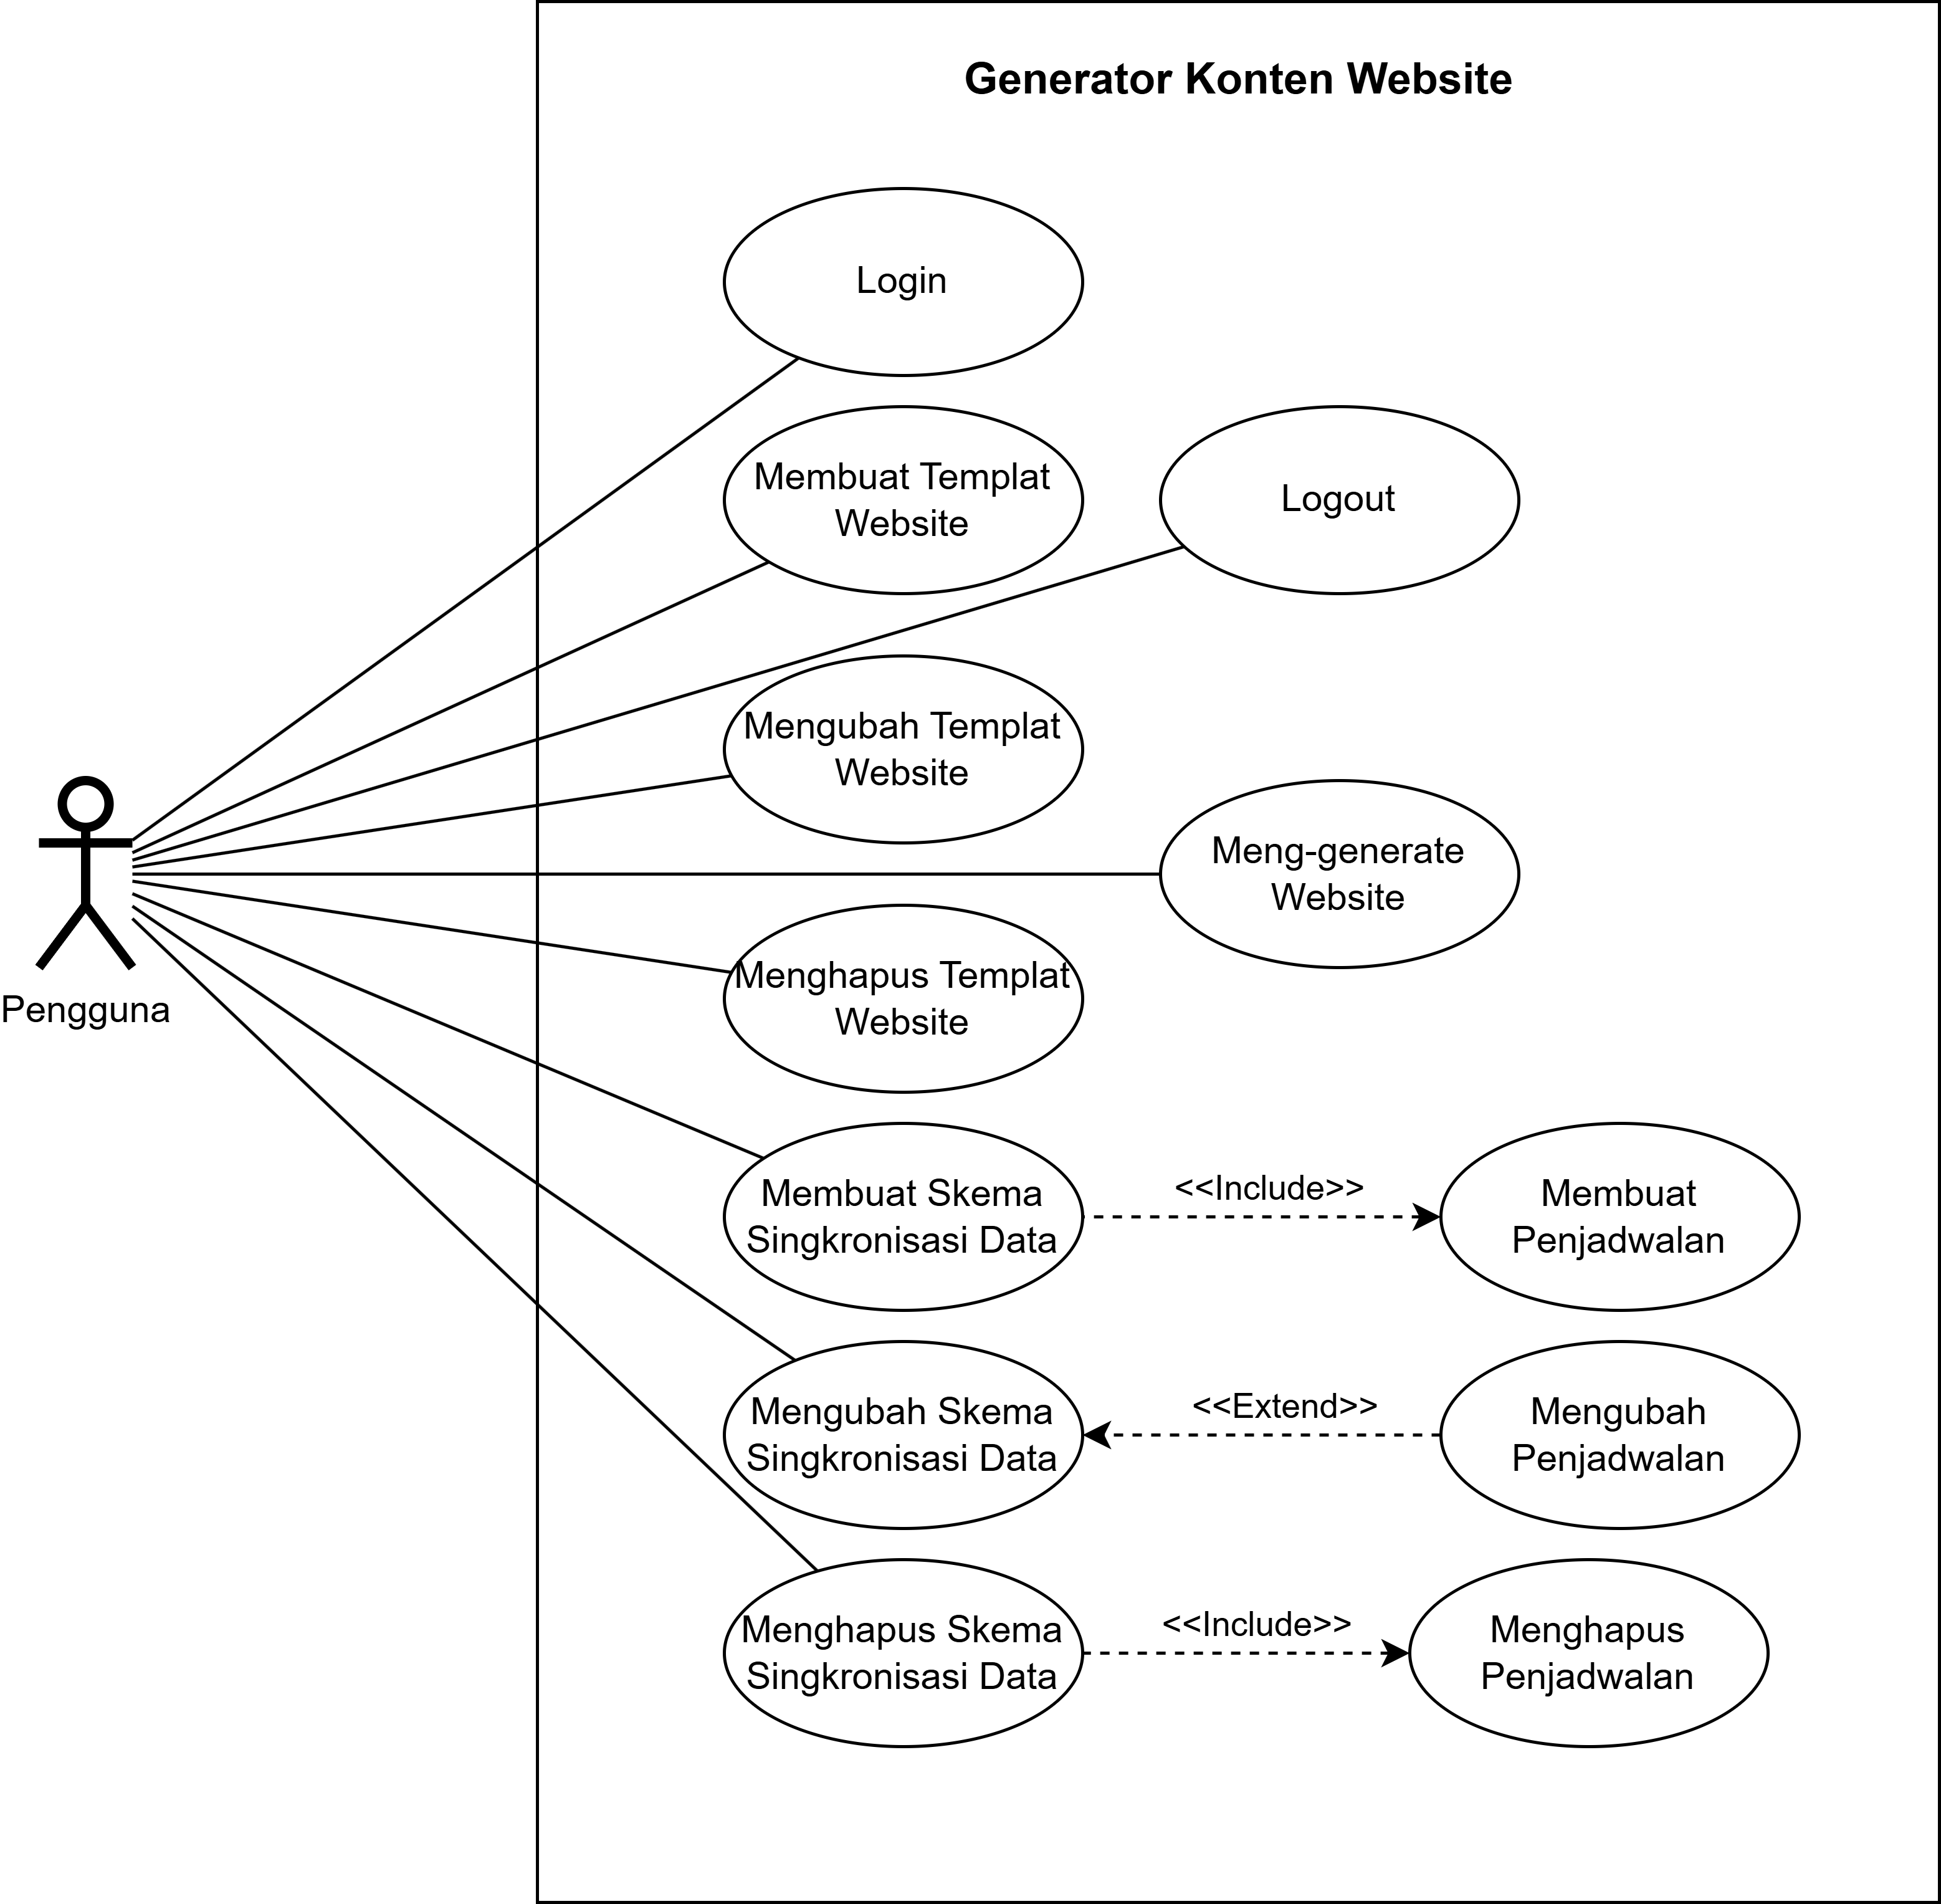
\includegraphics[width=0.8\linewidth]{figures/UseCaseDiagram.png}
        \caption{Diagram Use Case Generator Konten \textit{Website}}
        \label{fig:usecase-diagram}
    \end{figure}

    Diagram ini menunjukkan bahwa pengguna dapat melakukan berbagai tindakan, seperti mengelola templat, melakukan proses \textit{generate website}, mengatur sinkronisasi data, serta melakukan otentikasi.

    \item \textbf{Teknologi}\\
    Teknologi yang digunakan untuk mendukung implementasi fitur meliputi:
    \begin{enumerate}[label=\alph*.]
        \item \textbf{Bahasa Pemrograman}: JavaScript dengan \textit{runtime} Node.js.
        \item \textbf{Framework Backend}: Express.js untuk pengelolaan API dan server.
        \item \textbf{Library Backend}:
        \begin{itemize}
            \item \texttt{node-schedule}: Untuk penjadwalan sinkronisasi data.
            \item \texttt{joi}: Untuk validasi data.
            \item \texttt{sequelize}: Untuk manajemen basis data.
            \item \texttt{jsonwebtoken}: Untuk pengelolaan token otentikasi.
            \item \texttt{ejs}: Untuk pengelolaan templat halaman.
        \end{itemize}
        \item \textbf{Basis Data}: PostgreSQL untuk penyimpanan data yang terstruktur.
        \item \textbf{Frontend}: Dikembangkan menggunakan HTML, CSS, dan JavaScript tanpa menggunakan kerangka kerja (\textit{framework}).
        \item \textbf{Keamanan}: OAuth 2.0 Google untuk otentikasi dan kontrol akses pada aplikasi \textit{website}.
    \end{enumerate}
\end{enumerate} 

    \item \textbf{Melakukan perancangan pada basis data templat}\\
    {\bf Status :} Ada sejak rencana kerja tugas akhir.\\
    {\bf Hasil :}\\
    Untuk mendukung fitur-fitur yang telah ditetapkan, dirancang basis data yang dapat menyimpan templat \textit{website}, informasi terkait jadwal sinkronisasi, serta metadata tambahan yang diperlukan dalam sistem. Berikut adalah rincian dari perancangan basis data generator konten \textit{website}:
\begin{enumerate}[label*=\arabic*.,ref=\arabic*]
    \item Entitas
    \begin{enumerate}[label=\arabic*.]
        \item Entitas \textit{user}: Pada entitas ini akan berisi informasi dari pengguna yang dapat mengakses sistem.

        \item Entitas \textit{db\_config}: Entitas ini berisi informasi konfigurasi koneksi ke basis data, termasuk \textit{host, port}, nama basis data, jenis basis data, dan kredensial. Entitas ini digunakan untuk mendukung operasi sinkronisasi data antara sistem dan basis data eksternal.

        \item Entitas \textit{website}: Entitas ini berisi informasi tentang \textit{website} yang dihasilkan oleh sistem, termasuk nama, direktori penyimpanan, dan pembuatnya.

        \item Entitas \textit{asset\_static}: Entitas ini berisi informasi tentang aset-aset statis seperti \textit{file} HTML, CSS, atau JavaScript yang digunakan dalam \textit{website}.

        \item Entitas \textit{asset\_dynamic}: Entitas ini berisi informasi tentang data dinamis yang digunakan untuk menggantikan \textit{placeholder} pada entitas \textit{asset\_static}.

        \item Entitas \textit{job}: Pada entitas ini akan berisi informasi tentang tugas sinkronisasi data, termasuk jadwal, konfigurasi sumber data, dan tujuan data. Entitas ini berfungsi untuk mengelola proses sinkronisasi otomatis antara basis data eksternal dan sistem.

    \end{enumerate}


    \item Atribut
    \begin{enumerate}[label=\arabic*.]
        \item Entitas \textit{user}
        \vspace{-0.5em}
        \begin{table}[H]
            \centering
            \begin{tabular}{|p{3.25cm}|p{8cm}|}
                \hline
                \rowcolor[HTML]{DAE8FC} 
                {\color[HTML]{000000} Nama Atribut} & {\color[HTML]{000000} Keterangan}           \\ \hline
                user\_id                           & Menyimpan \textit{primary key} bertipe \textit{integer} untuk setiap pengguna. \\ \hline
                username                           & Menyimpan nama pengguna bertipe \textit{varchar} dengan panjang maksimal 200 karakter dan bersifat unik. \\ \hline
                email                              & Menyimpan alamat email pengguna bertipe \textit{varchar} dengan panjang maksimal 200 karakter dan bersifat unik. \\ \hline
                password                           & Menyimpan kata sandi pengguna bertipe \textit{text} yang sudah dalam bentuk terenkripsi. \\ \hline
                created\_at                        & Menyimpan waktu pembuatan pengguna bertipe \textit{big integer} yang disimpan sebagai \textit{epoch unix time}. \\ \hline
                updated\_at                        & Menyimpan waktu pembaruan terakhir pengguna bertipe \textit{big integer} yang disimpan sebagai \textit{epoch unix time} dan dapat bernilai \textit{null}. \\ \hline
            \end{tabular}
            \caption{Atribut dan keterangan pada entitas user}
            \label{tab:user_entity}
        \end{table}

        \item Entitas \textit{website}
        \vspace{-0.5em}
        \begin{table}[H]
            \centering
            \begin{tabular}{|p{3.25cm}|p{8cm}|}
                \hline
                \rowcolor[HTML]{DAE8FC} 
                {\color[HTML]{000000} Nama Atribut} & {\color[HTML]{000000} Keterangan}           \\ \hline
                website\_id                        & Menyimpan \textit{primary key} bertipe \textit{integer} untuk setiap \textit{website}. \\ \hline
                created\_by                        & Menyimpan \textit{foreign key} ke entitas \textit{user}, bertipe \textit{integer}, menunjukkan pengguna yang membuat \textit{website}. \\ \hline
                updated\_by                        & Menyimpan \textit{foreign key} ke entitas \textit{user}, bertipe \textit{integer}, menunjukkan pengguna yang terakhir memperbarui \textit{website}. Nilai dapat \textit{null} jika belum pernah diperbarui. \\ \hline
                name                               & Menyimpan nama \textit{website} bertipe \textit{varchar} dengan panjang maksimal 200 karakter. \\ \hline
                dir\_path                          & Menyimpan direktori penyimpanan file website bertipe \textit{varchar} dengan panjang maksimal 200 karakter. \\ \hline
                created\_at                        & Menyimpan waktu pembuatan \textit{websit}e bertipe \textit{big integer} yang disimpan sebagai \textit{epoch unix time}. \\ \hline
                updated\_at                        & Menyimpan waktu pembaruan terakhir \textit{website} bertipe \textit{big integer} yang disimpan sebagai \textit{epoch unix time} dan dapat bernilai \textit{null}. \\ \hline
            \end{tabular}
            \caption{Atribut dan keterangan pada entitas website}
            \label{tab:website_entity}
        \end{table}

        \item Entitas db\_config
        \vspace{-0.5em}
        \begin{table}[H]
            \centering
            \begin{tabular}{|p{3.25cm}|p{8cm}|}
                \hline
                \rowcolor[HTML]{DAE8FC} 
                {\color[HTML]{000000} Nama Atribut} & {\color[HTML]{000000} Keterangan}           \\ \hline
                db\_config\_id                     & Menyimpan \textit{primary key} bertipe \textit{integer} untuk setiap konfigurasi basis data. \\ \hline
                created\_by                        & Menyimpan \textit{foreign key} ke entitas \textit{user}, bertipe \textit{integer}, menunjukkan pengguna yang membuat konfigurasi basis data. \\ \hline
                website\_id                        & Menyimpan \textit{foreign key} ke entitas \textit{website}, bertipe \textit{integer}, menunjukkan \textit{website} pemilik basis data. \\ \hline
                updated\_by                        & Menyimpan \textit{foreign key} ke entitas \textit{user}, bertipe \textit{integer}, menunjukkan pengguna yang terakhir memperbarui konfigurasi basis data. Nilai dapat \textit{null} jika belum pernah diperbarui. \\ \hline
                host                               & Menyimpan alamat \textit{host} basis data bertipe \textit{varchar} dengan panjang maksimal 200 karakter. \\ \hline
                port                               & Menyimpan port yang digunakan untuk koneksi basis data bertipe \textit{integer}. \\ \hline
                db\_name                           & Menyimpan nama basis data bertipe \textit{varchar} dengan panjang maksimal 200 karakter. \\ \hline
                user                               & Menyimpan nama pengguna untuk koneksi basis data bertipe \textit{varchar} dengan panjang maksimal 200 karakter. \\ \hline
                password                           & Menyimpan kata sandi untuk koneksi basis data bertipe TEXT. \\ \hline
                type                               & Menyimpan jenis basis data bertipe \textit{enum} (\textit{'mysql', 'postgresql'}). \\ \hline
                created\_at                        & Menyimpan waktu pembuatan konfigurasi basis data bertipe \textit{big integer} yang disimpan sebagai \textit{epoch unix time.} \\ \hline
                updated\_at                        & Menyimpan waktu pembaruan konfigurasi basis data terakhir bertipe \textit{big integer} yang disimpan sebagai \textit{epoch unix time} dan dapat bernilai \textit{null}. \\ \hline
            \end{tabular}
            \caption{Atribut dan keterangan pada entitas db\_config}
            \label{tab:db_config_entity}
        \end{table}

        \item Entitas asset\_static
        \vspace{-0.5em}
        \begin{table}[H]
            \centering
            \begin{tabular}{|p{3.25cm}|p{8cm}|}
                \hline
                \rowcolor[HTML]{DAE8FC} 
                {\color[HTML]{000000} Nama Atribut} & {\color[HTML]{000000} Keterangan}           \\ \hline
                asset\_static\_id                  & Menyimpan \textit{primary key} bertipe \textit{integer} untuk setiap aset statis. \\ \hline
                created\_by                        & Menyimpan \textit{foreign key} ke entitas \textit{user}, bertipe \textit{integer}, menunjukkan pengguna yang membuat aset. \\ \hline
                updated\_by                        & Menyimpan \textit{foreign key} ke entitas \textit{user}, bertipe \textit{integer}, menunjukkan pengguna yang terakhir memperbarui aset. Nilai dapat \textit{null} jika belum pernah diperbarui. \\ \hline
                website\_id                        & Menyimpan \textit{foreign key} ke entitas \textit{website}, bertipe \textit{integer}, menunjukkan \textit{website} tempat aset ini berada. \\ \hline
                parent\_id                         & Menyimpan \textit{foreign key} ke entitas \textit{asset\_static}, bertipe \textit{integer}, menunjukkan aset induk jika aset ini adalah bagian dari folder. Nilai dapat \textit{null}. \\ \hline
                name                               & Menyimpan nama aset bertipe \textit{varchar} dengan panjang maksimal 200 karakter. \\ \hline
                type                               & Menyimpan jenis aset bertipe \textit{enum} (\textit{'file', 'folder'}). \\ \hline
                content                            & Menyimpan konten aset bertipe \textit{text}. Nilai dapat \textit{null}. \\ \hline
                placeholders                       & Menyimpan definisi placeholder dalam format JSONB. Nilai dapat \textit{null}. \\ \hline
                created\_at                        & Menyimpan waktu pembuatan aset bertipe \textit{big integer} yang disimpan sebagai \textit{epoch unix time}. \\ \hline
                updated\_at                        & Menyimpan waktu pembaruan terakhir aset bertipe \textit{big integer} yang disimpan sebagai \textit{epoch unix time} dan dapat bernilai \textit{null}. \\ \hline
            \end{tabular}
            \caption{Atribut dan keterangan pada entitas asset\_static}
            \label{tab:asset_static_entity}
        \end{table}

        \item Entitas asset\_dynamic
        \vspace{-0.5em}
        \begin{table}[H]
            \centering
            \begin{tabular}{|p{3.25cm}|p{8cm}|}
                \hline
                \rowcolor[HTML]{DAE8FC} 
                {\color[HTML]{000000} Nama Atribut} & {\color[HTML]{000000} Keterangan}           \\ \hline
                asset\_dynamic\_id                 & Menyimpan \textit{primary key} bertipe \textit{integer} untuk setiap aset dinamis. \\ \hline
                created\_by                        & Menyimpan \textit{foreign key} ke entitas \textit{user}, bertipe \textit{integer}, menunjukkan pengguna yang membuat aset dinamis. \\ \hline
                updated\_by                        & Menyimpan \textit{foreign key} ke entitas \textit{user}, bertipe \textit{integer}, menunjukkan pengguna yang terakhir memperbarui aset dinamis. Nilai dapat \textit{null} jika belum pernah diperbarui. \\ \hline
                asset\_static\_id                  & Menyimpan \textit{foreign key} ke entitas \textit{asset\_static}, bertipe \textit{integer}, menunjukkan aset statis yang terkait. \\ \hline
                placeholder\_values                & Menyimpan nilai pengganti untuk \textit{placeholder} dalam format JSONB. \\ \hline
                created\_at                        & Menyimpan waktu pembuatan aset dinamis bertipe \textit{big integer} yang disimpan sebagai \textit{epoch unix time}. \\ \hline
                updated\_at                        & Menyimpan waktu pembaruan terakhir aset dinamis bertipe \textit{big integer} yang disimpan sebagai \textit{epoch unix time} dan dapat bernilai \textit{null}. \\ \hline
            \end{tabular}
            \caption{Atribut dan keterangan pada entitas asset\_dynamic}
            \label{tab:asset_dynamic_entity}
        \end{table}

        \item Entitas job
        \vspace{-0.5em}
        \begin{table}[H]
            \centering
            \begin{tabular}{|p{3.25cm}|p{8cm}|}
                \hline
                \rowcolor[HTML]{DAE8FC} 
                {\color[HTML]{000000} Nama Atribut} & {\color[HTML]{000000} Keterangan}           \\ \hline
                job\_id                            & Menyimpan \textit{primary key} bertipe \textit{integer} untuk setiap tugas sinkronisasi. \\ \hline
                created\_by                        & Menyimpan \textit{foreign key} ke entitas \textit{user}, bertipe \textit{integer}, menunjukkan pengguna yang membuat tugas sinkronisasi. \\ \hline
                updated\_by                        & Menyimpan \textit{foreign key} ke entitas \textit{user}, bertipe \textit{integer}, menunjukkan pengguna yang terakhir memperbarui tugas sinkronisasi. Nilai dapat \textit{null} jika belum pernah diperbarui. \\ \hline
                db\_config\_id                     & Menyimpan \textit{foreign key} ke entitas \textit{db\_config}, bertipe \textit{integer}, menunjukkan konfigurasi basis data terkait. \\ \hline
                name                               & Menyimpan nama \textit{job}, bertipe \textit{varchar} dengan panjang maksimal 100 karakter. \\ \hline
                cron                               & Menyimpan format cron untuk penjadwalan tugas bertipe \textit{varchar} dengan panjang maksimal 20 karakter. \\ \hline
                count                               & Menyimpan jumlah \textit{job} yang sudah dijalankan bertipe \textit{integer}. \\ \hline
                tables                             & Menyimpan daftar tabel sumber dalam, bertipe JSONB. \\ \hline
                endpoint                           & Menyimpan URL API tujuan sinkronisasi bertipe \textit{varchar} dengan panjang maksimal 500 karakter. \\ \hline
                headers                            & Menyimpan header yang diperlukan untuk API tujuan dalam, bertipe JSONB. \\ \hline
                request\_format                    & Menyimpan format \textit{request} ke API tujuan dalam, bertipe JSONB. \\ \hline
                transform                          & Menyimpan aturan pemetaan antara data hasil ekstraksi dan struktur data yang diharapkan oleh API tujuan, bertipe JSONB. \\ \hline
                last\_run                          & Menyimpan waktu eksekusi terakhir, bertipe \textit{big integer} yang disimpan sebagai epoch unix time. Nilai dapat \textit{null} jika belum pernah dieksekusi. \\ \hline
                next\_run                          & Menyimpan waktu eksekusi berikutnya, bertipe \textit{big integer} yang disimpan sebagai epoch unix time. \\ \hline
                created\_at                        & Menyimpan waktu pembuatan tugas sinkronisasi bertipe \textit{big integer} yang disimpan sebagai epoch unix time. \\ \hline
                updated\_at                        & Menyimpan waktu pembaruan terakhir tugas sinkronisasi bertipe \textit{big integer} yang disimpan sebagai epoch unix time dan dapat bernilai \textit{null}. \\ \hline
            \end{tabular}
            \caption{Atribut dan keterangan pada entitas job}
            \label{tab:job_entity}
        \end{table}

\end{enumerate}


    \item Rancangan Entity Relationship Diagram (ERD)
        \begin{figure}[H]
            \centering
            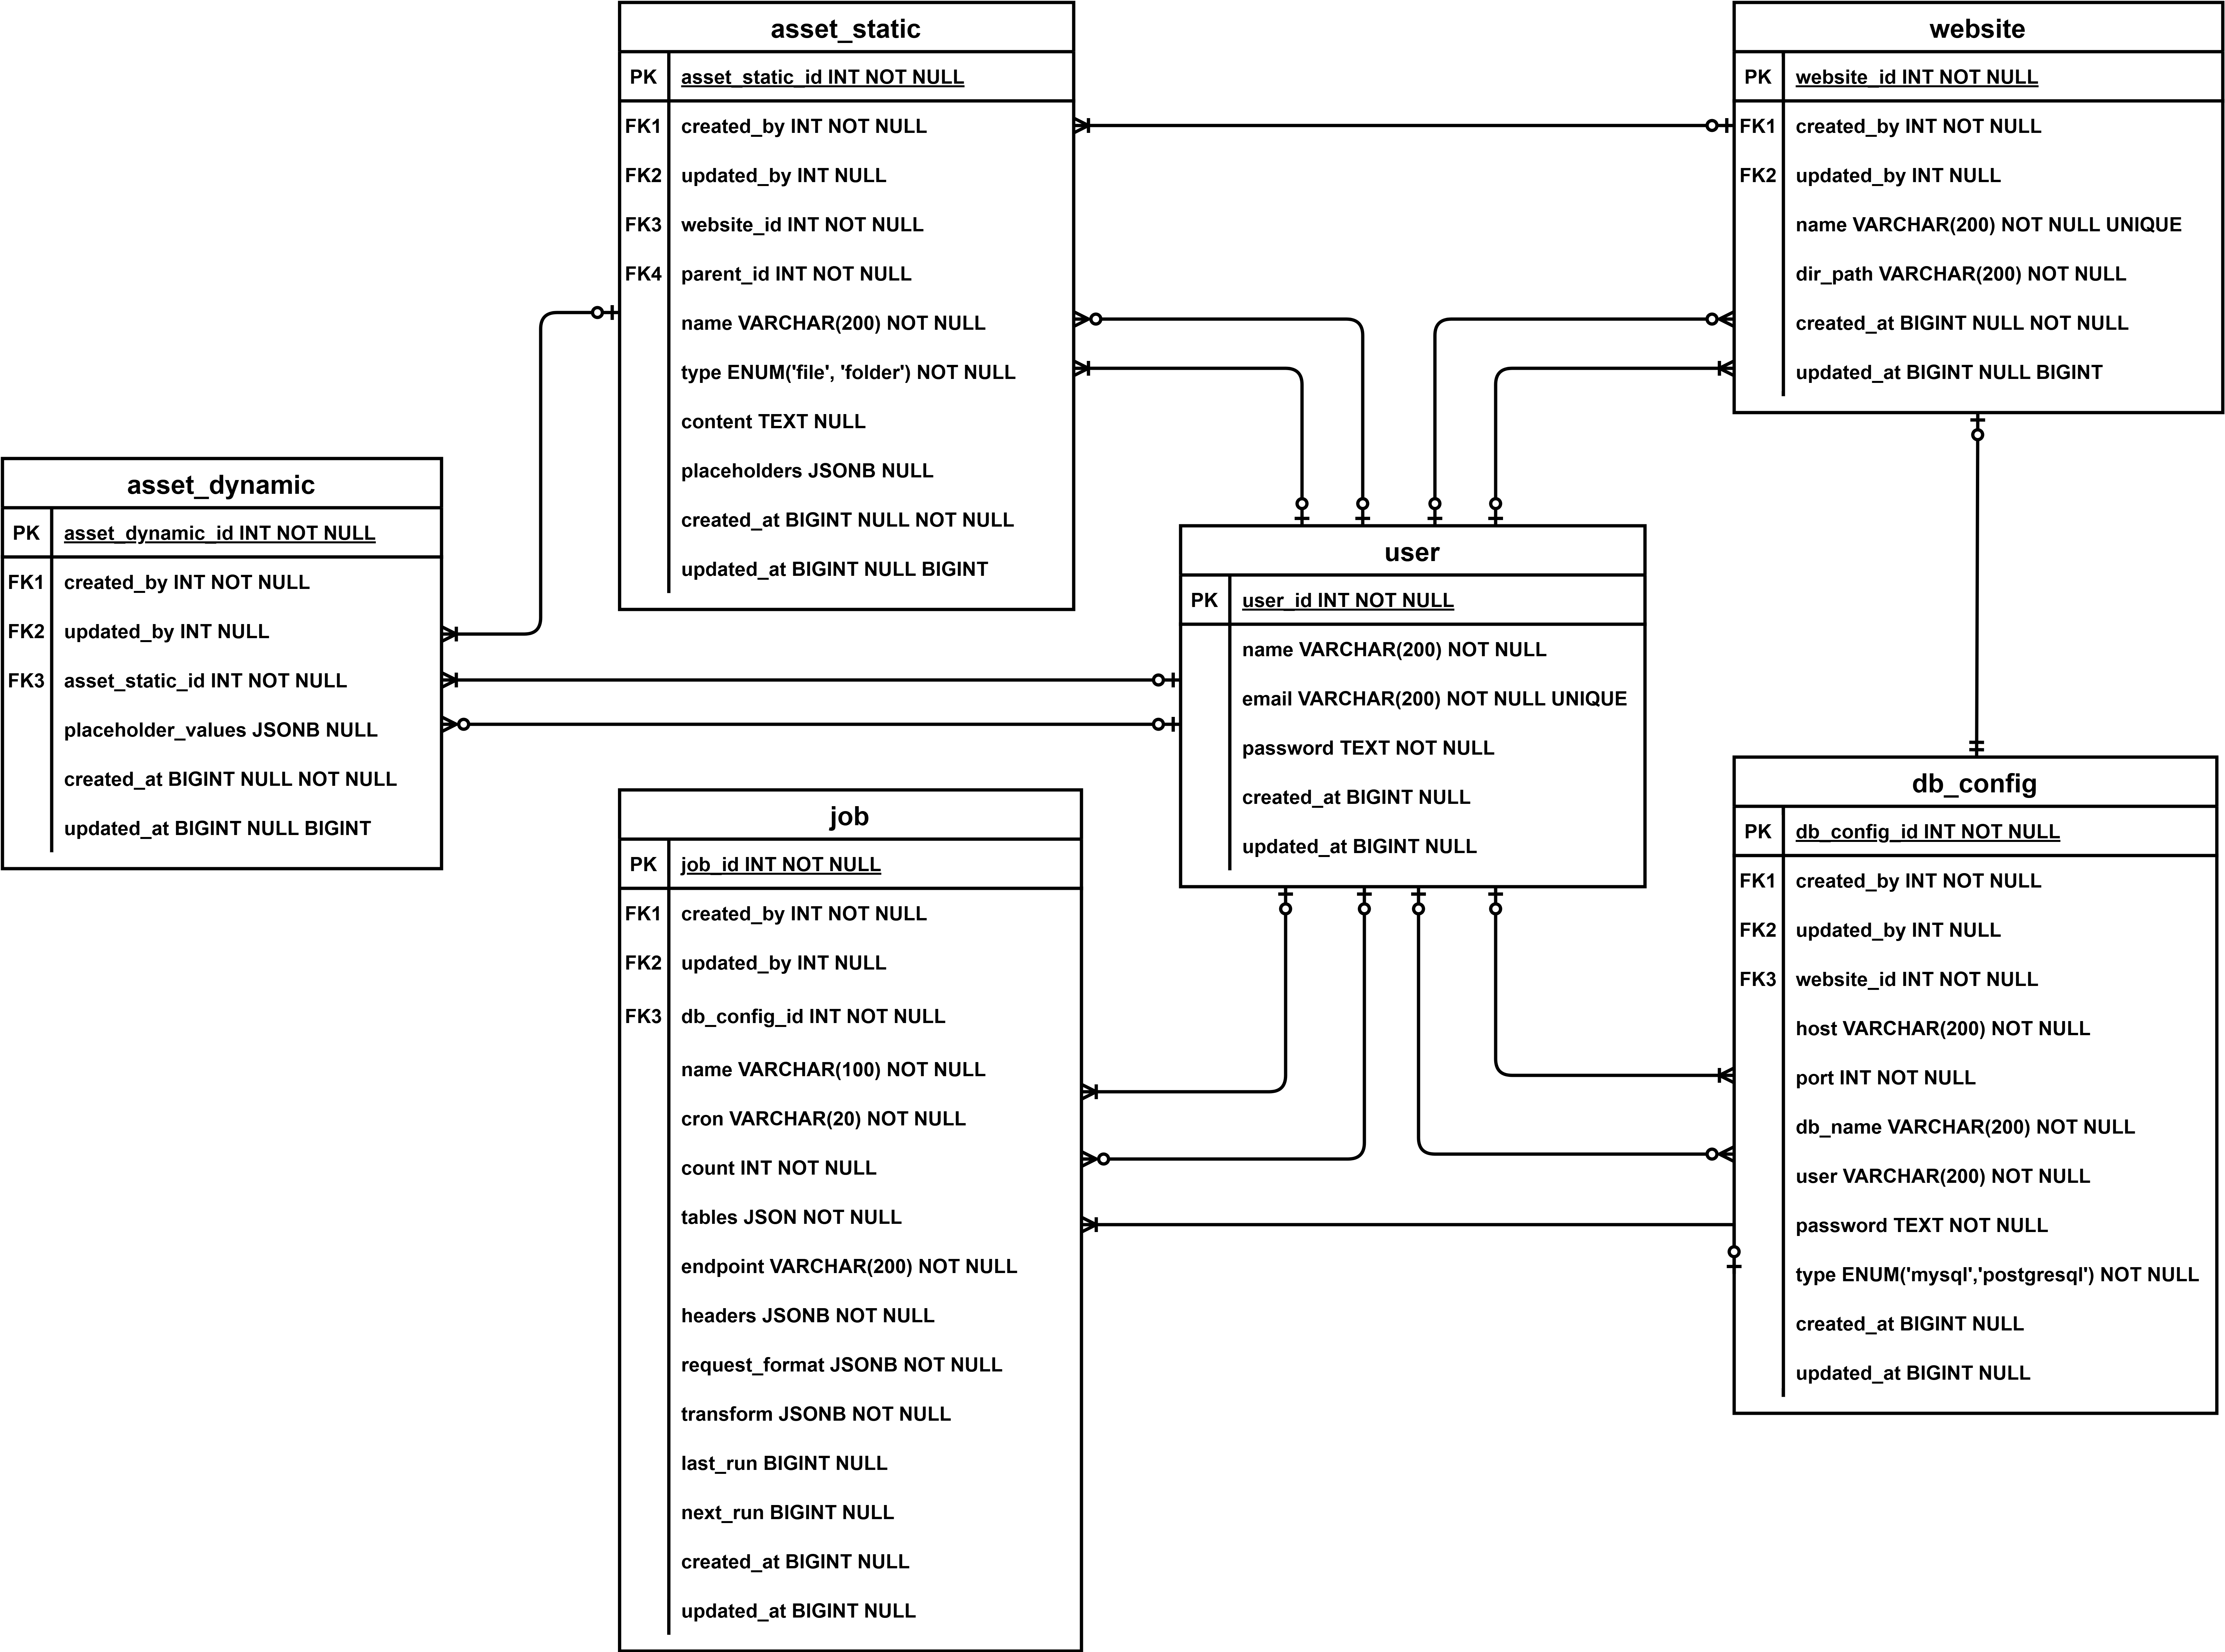
\includegraphics[width=0.8\linewidth]{figures/ERD-10.png}
            \caption{ERD Basis Data Templat}
            \label{fig:ERD-GeneratorKontenWebsite}
        \end{figure}

\end{enumerate}

    \item \textbf{Melakukan perancangan pada Generator Konten Website
    berbasis API}\\
    {\bf Status :} Ada sejak rencana kerja tugas akhir.\\
    {\bf Hasil :}\\
    \label{sec:perancangan-generator-konten-website}
    Perancangan sistem merupakan tahap penting dalam pengembangan perangkat lunak karena menjadi dasar bagi implementasi yang terarah. Pada tahap ini, dilakukan perancangan Generator Konten \textit{website} berbasis API untuk menyediakan solusi pengelolaan templat \textit{website} dan sinkronisasi data. Perancangan ini bertujuan untuk mendukung interoperabilitas, keamanan, dan keandalan sistem, serta menjadi pedoman teknis dalam proses implementasi berikutnya.

Arsitektur Generator Konten \textit{website} berbasis API terdiri dari enam komponen utama yang dapat dilihat pada Gambar \ref{fig:ArsitekturGeneratorKontenWebsite}, berikut adalah penjelasan setiap komponen:
\begin{enumerate}[label=\alph*.]
            
    \item \textbf{API Generator Konten \textit{website}}\\ 
        API Generator Konten \textit{website} merupakan inti dari sistem ini. Komponen ini bertanggung jawab untuk menangani berbagai operasi yang berkaitan dengan templat \textit{website} dan proses \textit{generate \textit{website}} berdasarkan permintaan pengguna.\\

        Berikut adalah spesifikasi teknis API Generator Konten \textit{website}:
        \begin{enumerate}[label=\arabic*.]
                
            \item \textbf{Arsitektur:} Representational State Transfer (REST)
                    
            \item \textbf{Teknologi:} Bahasa pemrograman Javascript dengan \textit{runtime Node.js} dan \textit{framework Express.js}
                        
            \item \textbf{Pendekatan Desain:} Modular
                    
        \end{enumerate}

    \item \textbf{API Aplikasi Internal}\\
        API Aplikasi Internal berfungsi sebagai penghubung antara sistem generator dan aplikasi lain di lingkungan internal. Komponen ini menyediakan layanan untuk pengambilan dan pemuatan data.\\
                
        Berikut adalah spesifikasi teknis API Aplikasi Internal:
        \begin{enumerate}[label=\arabic*.]
                
            \item \textbf{Arsitektur:} \textit{Representational State Transfer} (REST)
                    
            \item \textbf{Teknologi:} Bahasa pemrograman Javascript dengan \textit{runtime Node.js} dan \textit{framework Express.js}
                        
            \item \textbf{Pendekatan Desain:} Fokus pada \textit{endpoint} untuk pengambilan data (GET) dan pemuatan data (POST)
                    
        \end{enumerate}
            
    \item \textbf{Modul Sinkronisasi Data}\\
        Modul Sinkronisasi Data adalah komponen yang bertugas memastikan bahwa data yang ada di aplikasi internal selalu \textit{up-to-date} dengan data terbaru dari basis data aplikasi web.

        Berikut adalah fungsi utama dari Modul Sinkronisasi Data:
        \begin{enumerate}[label=\arabic*.]
                
            \item \textbf{Sinkronisasi Terjadwal:} Penjadwalan berbasis \textit{event-driven} menggunakan library \texttt{node-schedule}.
                    
            \item \textbf{Ekstraksi Data:} Mengambil data dari basis data aplikasi web berdasarkan konfigurasi yang ada dibasis data templat.
                    
            \item \textbf{Transformasi Data:} Melakukan validasi dan modifikasi pada data hasil ekstraksi agar sesuai dengan format yang diterima oleh API Aplikasi Internal.
                    
            \item \textbf{Load Data:} Mengirim data ke API Aplikasi Internal.
            \end{enumerate}

        Proses sinkronisasi data terdiri dari langkah-langkah berikut:
        \begin{enumerate}[label=\arabic*.]
            \item Modul membaca jadwal sinkronisasi dari entitas \textit{job}.
            \item Modul mengakses konfigurasi koneksi basis data dari entitas \textit{db\_config}.
            \item Modul melakukan ekstraksi data dari tabel yang ditentukan di basis data aplikasi web.
            \item Data yang diekstrak divalidasi dan dimodifikasi agar sesuai dengan struktur data yang dibutuhkan oleh API tujuan berdasarkan aturan yang sudah didefinisikan di entitas \textit{job}.
            \item Data yang telah diproses dikirim ke API Aplikasi Internal menggunakan metode \texttt{POST}.
        \end{enumerate}
        
    \item \textbf{Basis Data Templat}\\ 
        Basis Data Templat adalah pusat penyimpanan templat \textit{website} dan informasi tambahan yang terkait. Basis data ini dirancang menggunakan \textit{Relational Database Management System} (RDBMS) PostgreSQL.

    \item \textbf{Basis Data Aplikasi Web}\\
        Basis Data Aplikasi Web digunakan untuk menyimpan data dari aplikasi web yang dihasilkan oleh Generator Konten \textit{website}. Basis data ini dirancang menggunakan \textit{Relational Database Management System} (RDBMS), seperti PostgreSQL atau MySQL, tergantung pada kebutuhan proyek.

    \item \textbf{Pengguna}\\
        Pengguna adalah entitas yang berinteraksi dengan API Generator Konten \textit{website} melalui \textit{endpoint} yang disediakan. Mereka dapat mengelola templat, meminta generasi \textit{website}, serta memantau status proses melalui antarmuka yang tersedia.
            
\end{enumerate}

\begin{figure}[H]
    \centering
    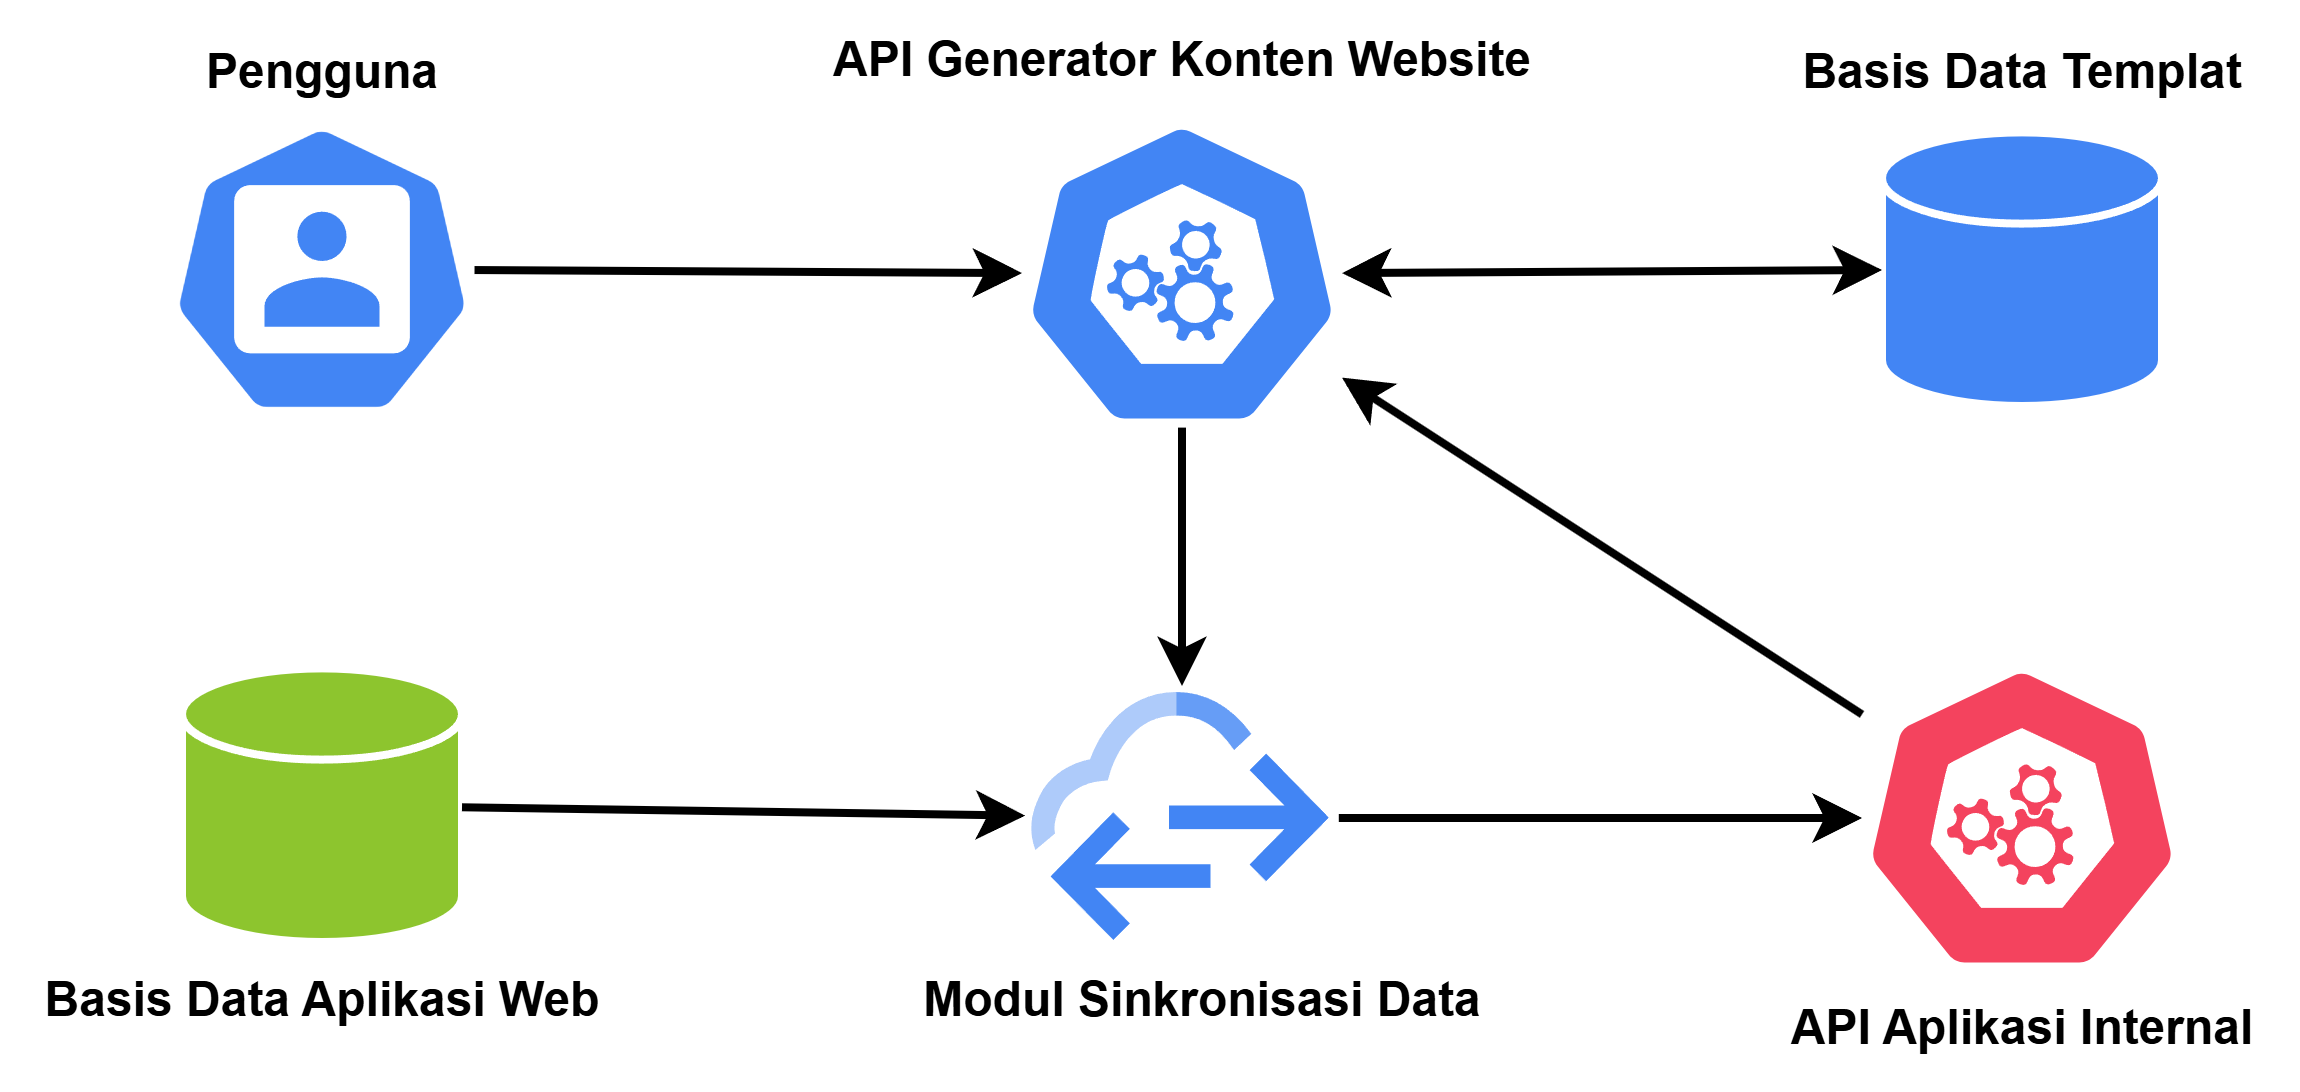
\includegraphics[width=0.8\linewidth]{figures/ArsitekturGeneratorKontenWebsite.png}
    \caption{Arsitektur Generator Konten \textit{website}}
    \label{fig:ArsitekturGeneratorKontenWebsite}
\end{figure}
 

    \item \textbf{Melakukan perancangan pada modul sinkronisasi data}\\
    {\bf Status :} Ada sejak rencana kerja tugas akhir.\\
    {\bf Hasil :}\\
    Rancangan Modul Sinkronisasi Data telah dibahas pada bagian \ref{sec:perancangan-generator-konten-website} sebagai salah satu komponen utama dari Generator Konten Website berbasis API. Modul ini dirancang untuk memastikan bahwa data yang ada di aplikasi internal selalu \textit{up-to-date} dengan data terbaru dari basis data aplikasi web. Mekanisme sinkronisasi ini mencakup penjadwalan otomatis, proses ekstraksi data, validasi dan transformasi data, serta pengiriman data ke API Aplikasi Internal.


    \item \textbf{Melakukan perancangan pada SSO OAuth 2.0}\\
    {\bf Status :} Ada sejak rencana kerja tugas akhir.\\
    {\bf Hasil :}\\
    Pada tahap ini, dirancang implementasi otentikasi berbasis \textit{Single Sign-On} (SSO) menggunakan protokol OAuth 2.0 yang disediakan oleh Google. SSO ini dirancang untuk mempermudah proses otentikasi pengguna di aplikasi web hasil \textit{generate}, sehingga pengguna dapat menggunakan kredensial Google mereka tanpa perlu membuat akun baru. Selain itu, implementasi ini memastikan bahwa hanya pengguna yang telah terdaftar dalam basis data aplikasi web hasil \textit{generate} yang diizinkan untuk mengakses sistem.

Rancangan teknis meliputi teknologi yang digunakan, alur otentikasi, serta spesifikasi implementasi, sebagai berikut:

\begin{enumerate}[label*=\arabic*.,ref=\arabic*]

    \item \textbf{Teknologi yang Digunakan}\\
    SSO menggunakan OAuth 2.0 Google dengan memanfaatkan layanan Google Identity Platform. Teknologi yang dipilih meliputi:
    \begin{itemize}
        \item \texttt{googleapis}: \textit{Library} untuk mengelola permintaan otentikasi OAuth 2.0.
        \item \texttt{jsonwebtoken} (JWT): Untuk memvalidasi token ID yang diterima dari Google.
        \item HTTPS: Semua komunikasi dilakukan melalui protokol yang aman untuk memastikan keamanan data.
    \end{itemize}

    \item \textbf{Alur Otentikasi OAuth 2.0}\\
    Proses otentikasi OAuth 2.0 yang dirancang adalah sebagai berikut:
    \begin{enumerate}[label=\alph*.]
        \item \textbf{Permintaan otentikasi:}\\
        Pengguna diarahkan ke endpoint otentikasi Google melalui URL otorisasi yang mencakup parameter seperti \textit{client\_id}, \textit{redirect\_uri}, \textit{response\_type}, dan \textit{scope}.
        
        \item \textbf{Penerimaan Kode Otorisasi:}\\
        Setelah pengguna berhasil login ke Google, Google mengembalikan kode otorisasi ke \textit{redirect\_uri} aplikasi.

        \item \textbf{Pertukaran Kode Otorisasi dengan Token Akses:}\\
        Aplikasi web hasil \textit{generate} mengirimkan kode otorisasi ke endpoint token Google untuk mendapatkan token akses (\textit{access\_token}) dan token ID (\textit{id\_token}).

        \item \textbf{Validasi Token ID:}\\
        Token ID yang diterima dari Google divalidasi menggunakan \textit{library} \textit{jsonwebtoken} untuk memastikan keabsahan dan integritasnya.

        \item \textbf{Validasi Email terhadap Basis Data:}\\
        Email yang diambil dari token ID dibandingkan dengan data di basis data aplikasi web hasil \textit{generate}. Jika email ditemukan, akses diberikan. Jika tidak, pengguna diberi pesan bahwa akses ditolak.

        \item \textbf{Akses Pengguna:}\\
        Setelah validasi berhasil, pengguna dianggap terotentikasi dan diberikan akses ke aplikasi.
    \end{enumerate}
\end{enumerate}


    \item \textbf{Melakukan perancangan pada templat website}\\
    {\bf Status :} Ada sejak rencana kerja tugas akhir.\\
    {\bf Hasil :}\\
    Templat \textit{website} dirancang untuk menjadi dasar dalam proses \textit{generate website} oleh Generator Konten \textit{Website} berbasis API. Perancangan templat ini bertujuan untuk menyediakan struktur yang fleksibel, mudah digunakan, dan mampu mendukung berbagai kebutuhan pengguna. Selain itu, templat harus memungkinkan personalisasi dengan mengganti \textit{placeholder} atau data dinamis sesuai konfigurasi pengguna.

Berikut adalah komponen-komponen dari sebuah templat:
\begin{enumerate}[label=\alph*.]
    \item \textbf{Website}\\
        Komponen ini merupakan inti dari sebuah templat \textit{website}. Pada komponen ini, pengguna menentukan:
        \begin{itemize}
            \item Nama \textit{website} templat, yang akan menjadi identitas unik dari templat.
            \item Direktori penyimpanan hasil \textit{generate} dari templat, yang menentukan lokasi folder \textit{output} setelah proses \textit{generate website}.
        \end{itemize}
        \textit{Website} juga berfungsi sebagai entitas utama yang mengelola hubungan dengan komponen lainnya, seperti aset statis, aset dinamis, dan konfigurasi basis data jika diperlukan.

    \item \textbf{Basis Data}\\
        Komponen ini merupakan bagian yang opsional, tergantung pada jenis \textit{website} apakah membutuhkan basis data atau tidak. Jika basis data diperlukan, pengguna dapat mendefinisikan spesifikasi koneksi ke basis data. Spesifikasi yang dapat ditentukan meliputi:
        \begin{itemize}
            \item \textbf{Host basis data}: Alamat server basis data.
            \item \textbf{Port}: Nomor \textit{port} yang digunakan untuk koneksi ke server.
            \item \textbf{Nama basis data}: Nama basis data yang akan digunakan.
            \item \textbf{Jenis basis data}: Format basis data seperti MySQL, PostgreSQL, atau lainnya.
            \item \textbf{Kredensial pengguna}: Informasi \textit{username} dan \textit{password} untuk otentikasi.
        \end{itemize}
        Basis data ini dapat digunakan untuk mendukung operasi dinamis pada \textit{website} hasil \textit{generate}, seperti pengelolaan data pengguna atau konten yang berubah-ubah.

    \item \textbf{Aset Statis}\\
        Komponen ini merupakan bagian yang menentukan struktur dan isi \textit{file} dalam templat. Aset statis dapat berupa folder atau \textit{file}. Jika sebuah aset berupa \textit{file}, pengguna harus memasukkan isi \textit{file} tersebut, dan bagian-bagian yang dapat diganti dengan aset dinamis harus diberi penanda menggunakan \textit{placeholder}. \textit{Placeholder} adalah penanda khusus yang nantinya akan diganti dengan data dinamis saat proses \textit{generate website}.

        Berikut adalah contoh aset statis dengan \textit{placeholder}:
        \begin{lstlisting}[language=Javascript,caption={Contoh Aset Statis}]
const express = require('express');
const router = express.Router();
const {{MODEL_NAME}} = require('../models/{{MODEL_NAME}}');

router.get('/', async (req, res) => {
const {{VARIABLE_NAME}} = await {{MODEL_NAME}}.findAll();
    res.render('pages/home', { {{VARIABLE_NAME}} });
});

module.exports = router;
\end{lstlisting}
        
        Pada contoh di atas:
        \begin{itemize}
            \item \texttt{\{\{MODEL\_NAME\}\}} adalah \textit{placeholder} untuk nama model dalam aplikasi.
            \item \texttt{\{\{VARIABLE\_NAME\}\}} adalah \textit{placeholder} untuk nama variabel yang digunakan.
        \end{itemize}
        \textit{Placeholder} ini memungkinkan \textit{file} statis untuk disesuaikan sesuai kebutuhan pengguna.

    \item \textbf{Aset Dinamis}\\
        Komponen ini merupakan bagian yang menentukan nilai pengganti untuk \textit{placeholder} yang ada di aset statis. Pengguna mendefinisikan aset dinamis dengan memilih \textit{placeholder} tertentu dari aset statis dan memberikan nilai penggantinya. Nilai ini akan digunakan saat proses \textit{generate website} untuk menggantikan \textit{placeholder}.

        Berikut adalah contoh aset dinamis yang menggantikan \textit{placeholder} pada contoh aset statis di atas:
        \begin{lstlisting}[language=Javascript,caption={Contoh Aset Dinamis}]
{
    "MODEL_NAME": "User",
    "VARIABLE_NAME": "getUser"
}
\end{lstlisting}

        Dalam proses \textit{generate website}, \textit{placeholder} \texttt{\{\{MODEL\_NAME\}\}} akan digantikan oleh nilai \texttt{"User"} dan \textit{placeholder} \texttt{\{\{VARIABLE\_NAME\}\}} akan digantikan oleh nilai \texttt{"getUser"}.
\end{enumerate}


    \item \textbf{Melakukan pengembangan generator konten website berbasis API}\\
    {\bf Status :} Ada sejak rencana kerja tugas akhir.\\
    {\bf Hasil :}\\
    Pengembangan Generator Konten \textit{Website} berbasis API bertujuan untuk merealisasikan sistem yang dirancang, menyediakan antarmuka API untuk pengelolaan templat, dan menghasilkan \textit{website} berdasarkan templat pilihan pengguna.

\begin{enumerate}[label*=\arabic*.,ref=\arabic*]
    \item Lingkungan Pengembangan
        \begin{itemize}
            \item \textbf{Bahasa Pemrograman:} JavaScript.
            \item \textbf{Runtime:} Node.js.
            \item \textbf{Framework Backend:} Express.js.
            \item \textbf{ORM:} \textit{Sequelize} untuk PostgreSQL.
            \item \textbf{Pustaka:}
                \begin{itemize}
                    \item \texttt{body-parser}: \textit{Middleware} untuk \textit{parsing body request.}
                    \item \texttt{dotenv}: Manajemen konfigurasi lingkungan.
                    \item \texttt{joi}: Validasi data.
                    \item \texttt{jsonwebtoken}: Otentikasi berbasis token.
                    \item \texttt{pg} dan \texttt{pg-hstore}: Koneksi PostgreSQL.
                \end{itemize}
        \end{itemize}
        
    \item Struktur Proyek\\
        Struktur proyek dirancang untuk mendukung modularitas dan kemudahan pengelolaan kode. Berikut adalah struktur direktori proyek:

        \begin{itemize}
            \item \textbf{config/}: Berisi file konfigurasi seperti koneksi basis data.
            \item \textbf{controllers/}: Berisi fungsi untuk menangani permintaan dan respons API.
            \item \textbf{routes/}: Mendefinisikan \textit{endpoint} API dan menghubungkannya dengan \textit{controller}.
            \item \textbf{models/}: Berisi definisi tabel basis data menggunakan Sequelize.
            \item \textbf{repositories/}: Mengabstraksi \textit{query} basis data untuk digunakan oleh \textit{service}.
            \item \textbf{services/}: Berisi logika bisnis, seperti pengelolaan templat atau proses \textit{generate website.}
            \item \textbf{middlewares/}: \textit{Middleware} untuk validasi data, otentikasi JWT, dll.
            \item \textbf{utils/}: Berisi fungsi pendukung yang digunakan di berbagai bagian sistem.
        \end{itemize}

        
    \item Implementasi Fitur
        \begin{enumerate}[label=\alph*.]
            \item \textbf{Pengelolaan Templat \textit{Website}}\\
            API ini memungkinkan pengguna untuk mengelola templat dengan menambahkan, membaca, memperbarui, dan menghapus templat. Contoh implementasi \textit{endpoint} untuk menambahkan templat baru:
            \begin{lstlisting}[language=Javascript,caption={Asset Static Route}]
const express = require("express");
const {
	AssetStaticController,
} = require("../controllers/AssetStaticController");
const { Authorization } = require("../middlewares/Authorization");
const router = express.Router();

router.use("/", Authorization.decryption());

router.get("/", AssetStaticController.getAll);
router.get("/:id", AssetStaticController.getOne);
router.post("/", AssetStaticController.post);
router.patch("/:id", AssetStaticController.patch);
router.delete("/:id", AssetStaticController.delete);

module.exports = router;
\end{lstlisting}

            \item \textbf{\textit{Generate Website}}\\
            API ini memungkinkan pengguna menghasilkan \textit{website} berdasarkan templat. Proses melibatkan penggabungan aset statis dan dinamis, serta penyimpanan hasil di direktori yang telah ditentukan. Contoh kode:
            \begin{lstlisting}[language=Javascript,caption={Generate Website Service}]
const { WebsiteRepository } = require("../repositories/WebsiteRepository");
const fs = require("fs");
const path = require("path");

// Fungsi untuk mendekode Base64
function decodeBase64(content) {
	return Buffer.from(content, "base64").toString("utf-8");
}

class GenerateService {
	static async generate(dataGenerate) {
		try {
			const findGenerate = await WebsiteRepository.readForGenerate(
				dataGenerate
			);

			const basePath = path.resolve(
				__dirname,
				"..",
				findGenerate.website.dir_path
			);

			await this.processAssets(findGenerate.assets, basePath);

			return { success: true };
		} catch (error) {
			throw error;
		}
	}

	static async processAssets(assets, basePath) {
		for (const asset of assets) {
			const assetPath = path.join(basePath, asset.name);

			if (asset.type === "folder") {
				// Buat folder jika belum ada
				if (!fs.existsSync(assetPath)) {
					fs.mkdirSync(assetPath, { recursive: true });
					console.log(`Folder created: ${assetPath}`);
				}
				// Rekursi untuk anak-anak dari folder ini
				if (asset.children && asset.children.length > 0) {
					await this.processAssets(asset.children, assetPath);
				}
			} else if (asset.type === "file") {
				// Decode content jika ada
				let content = asset.content ? decodeBase64(asset.content) : "";

				// Ganti placeholder dengan placeholder_values
				if (asset.placeholder_values) {
					for (const [key, value] of Object.entries(asset.placeholder_values)) {
						const placeholder = new RegExp(`{{${key}}}`, "g");
						content = content.replace(placeholder, value);
					}
				}

				// Handle backticks dalam konten
				if (content.includes("`")) {
					content = content.replace(/`/g, "`"); // Pastikan backticks tetap aman
				}

				// Tulis konten ke file
				fs.writeFileSync(assetPath, content, "utf-8");
				console.log(`File created: ${assetPath}`);
			} else {
				console.warn(`Unknown asset type: ${asset.type} for ${asset.name}`);
			}
		}
	}
}

module.exports = { GenerateService };
\end{lstlisting}

            \item \textbf{Validasi Data}\\
            Validasi dilakukan menggunakan pustaka \texttt{joi} untuk memastikan data sesuai dengan skema. Contoh implementasi validasi:
           \begin{lstlisting}[language=Javascript,caption={Validasi Masukan Data Aset Statis}]
createAssetStatic(data) {
   const schema = Joi.object({
      website_id: Joi.number().integer().min(1).required().messages({
         "number.base": "Website ID must be a number.",
         "number.integer": "Website ID must be an integer.",
         "number.min": "Website ID must be at least 1.",
         "any.required": "Website ID is required.",
      }),
      parent_id: Joi.number().integer().min(1).allow(null).optional().messages({
         "number.base": "Parent ID must be a number.",
         "number.integer": "Parent ID must be an integer.",
         "number.min": "Parent ID must be at least 1.",
      }),
      name: Joi.string().max(200).required().messages({
         "string.base": "Name must be a string.",
         "string.empty": "Name cannot be empty.",
         "string.max": "Name cannot exceed 200 characters.",
         "any.required": "Name is required.",
      }),
      type: Joi.string().valid("file", "folder").required().messages({
         "string.base": "Type must be a string.",
         "any.only": "Type must be either 'file' or 'folder'.",
         "any.required": "Type is required.",
      }),
      content: Joi.string().allow(null).optional().messages({
         "string.base": "Content must be a string.",
      }),
      placeholders: Joi.object().allow(null).optional().messages({
         "object.base": "Placeholders must be an object or null.",
      }),
   }).required();

   return schema.validate(data, { abortEarly: false });
}
\end{lstlisting}
        \end{enumerate}
        
\end{enumerate}

    \item \textbf{Melakukan pengembangan modul sinkronisasi data}\\
    {\bf Status :} Ada sejak rencana kerja tugas akhir.\\
    {\bf Hasil :}\\
    Modul Sinkronisator Data dikembangkan untuk memastikan bahwa data antara basis data aplikasi web hasil \textit{generate} dan aplikasi internal tetap sinkron secara otomatis berdasarkan jadwal yang telah ditentukan. Modul ini dirancang dengan pendekatan modular dan fleksibel untuk mendukung kebutuhan sinkronisasi data yang kompleks.

\begin{enumerate}[label*=\arabic*.,ref=\arabic*]
    \item \textbf{Lingkungan Pengembangan}\\
    Modul ini dibangun menggunakan teknologi berikut:
    \begin{itemize}
        \item \texttt{axios}: Untuk melakukan HTTP \textit{/} ke API aplikasi internal.
        \item \texttt{node-schedule}: Untuk menjadwalkan sinkronisasi secara otomatis berdasarkan ekspresi \texttt{cron}.
    \end{itemize}

    \item \textbf{Implementasi Fitur}\\
    Implementasi modul mencakup dua fitur utama, yaitu penjadwalan sinkronisasi dan sinkronisasi data.
        \begin{enumerate}[label=\alph*.]
            \item \textbf{Penjadwalan Sinkronisasi}\\
            Penjadwalan sinkronisasi dilakukan menggunakan pustaka \texttt{node-schedule}. Setiap pekerjaan (\textit{job}) disimpan dalam objek konfigurasi yang mencakup nama, jadwal \texttt{cron}, dan detail sinkronisasi. Penjadwalan ini memastikan bahwa sinkronisasi berjalan secara otomatis sesuai dengan waktu yang telah ditentukan.

            Berikut adalah contoh implementasi penjadwalan sinkronisasi:
            \begin{lstlisting}[language=Javascript,caption={Penjadwalan Job}]
const createJob = async (dataJob) => {
	try {
		const job = schedule.scheduleJob(
			dataJob.name,
			dataJob.cron,
			async function () {
				try {
					await etl(dataJob);

					const currDate = new Date().toLocaleString();
					console.log(`Job ${dataJob.name} selesai pada ${currDate}`);
				} catch (etlError) {
					console.error(
						`Error dalam ETL untuk job ${dataJob.name}: ${etlError.message}`
					);
				}
			}
		);

		JOBS[dataJob.name] = job;
	} catch (error) {
		throw error;
	}
};
\end{lstlisting}

            \item \textbf{Sinkronisasi Data}\\
            Sinkronisasi data dilakukan dalam tiga tahap utama: \textit{Extract}, \textit{Transform}, dan \textit{Load} (ETL). Setiap tahap dirancang sebagai fungsi modular yang dapat digunakan kembali.

                \begin{itemize}
                    \item \textit{Extract Data}\\
                    Tahap ini bertugas mengambil data dari basis data aplikasi web hasil \textit{generate}. Koneksi ke basis data dilakukan menggunakan konfigurasi yang telah ditentukan. Data diekstrak dari tabel yang relevan sesuai kebutuhan sinkronisasi.

                    Berikut adalah implementasi fungsi \textit{Extract}:
                    \begin{lstlisting}[language=Javascript,caption={Extract Data}]
async function extract(dataJob) {
	try {
		console.log("Melakukan ekstraksi data...");

		const connection = await connectToDatabase(dataJob.source_db);

		const tables = dataJob.tables;
		const extractedData = {};

		for (const table of tables) {
			console.log(`Mengambil data dari tabel: ${table}`);
			extractedData[table] = await connection.query(`SELECT * FROM ${table}`);
		}

		return extractedData;
	} catch (error) {
		throw new Error(`Gagal mengekstrak data: ${error.message}`);
	}
}
\end{lstlisting}

                    \item \textit{Transform Data}\\
                    Data hasil ekstraksi diubah ke dalam format yang dapat diterima oleh API aplikasi internal. Proses transformasi dilakukan berdasarkan aturan (\textit{mapping rules}) yang didefinisikan dalam konfigurasi sinkronisasi.

                    Berikut adalah implementasi fungsi \textit{Transform}:
                    \begin{lstlisting}[language=Javascript,caption={Transform Data}]
async function transform(dataJob, data) {
	try {
		const transformRules = dataJob.transform;
		const transformedData = {};

		for (const [table, rows] of Object.entries(data)) {
			transformedData[table] = rows.map((row) => {
				const transformedRow = {};
				const rules = transformRules[table];

				for (const [sourceField, targetField] of Object.entries(rules)) {
					transformedRow[targetField] = row[sourceField];
				}

				return transformedRow;
			});
		}

		return transformedData;
	} catch (error) {
		throw new Error(`Gagal mentransformasi data: ${error.message}`);
	}
}
\end{lstlisting}

                    \item \textit{Load Data}\\
                    Data yang telah ditransformasi dikirimkan ke API aplikasi internal menggunakan pustaka \texttt{axios}. Proses ini mencakup validasi token autentikasi dan pengiriman data ke \textit{endpoint} yang ditentukan.

                    Berikut adalah implementasi fungsi \textit{Load}:
                    \begin{lstlisting}[language=Javascript,caption={Load Data}]
async function load(dataJob, data) {
	try {
		const endpoint = dataJob.endpoint;
		const headers = dataJob.headers;

		for (const [table, rows] of Object.entries(data)) {
			await axios.post(endpoint, rows, { headers });
		}
	} catch (error) {
		throw new Error(`Gagal memuat data ke API tujuan: ${error.message}`);
	}
}
\end{lstlisting}
                \end{itemize}
        \end{enumerate}
\end{enumerate}


    \item \textbf{Melakukan pengujian fungsional pada generator konten website}\\
    {\bf Status :} Ada sejak rencana kerja tugas akhir.\\
    {\bf Hasil :}\\
    Pengujian fungsional bertujuan untuk memastikan bahwa setiap fitur dari Generator Konten Website berbasis API berfungsi sesuai dengan spesifikasi yang telah ditentukan. Pengujian dilakukan dengan menguji endpoint API menggunakan skenario pengujian yang mencakup berbagai kondisi masukan dan keluaran.

\begin{enumerate}[label*=\arabic*.,ref=\arabic*]

    \item \textbf{Tujuan Pengujian}\\
    Pengujian dilakukan untuk memastikan:
    \begin{itemize}
        \item Setiap endpoint API bekerja sesuai dengan spesifikasi yang telah ditentukan.
        \item Validasi data masukan dilakukan dengan benar oleh API.
        \item Proses \textit{generate website} menghasilkan output yang sesuai dengan konfigurasi templat.
        \item Kesalahan dalam implementasi dapat diidentifikasi dan diperbaiki dengan cepat.
    \end{itemize}

    \item \textbf{Lingkungan Pengujian}\\
    Pengujian dilakukan pada lingkungan pengembangan dengan konfigurasi sebagai berikut:
    \begin{itemize}
        \item \textbf{Alat Pengujian:} Postman untuk Windows v11.22.1
        \item \textbf{Basis Data:} PostgreSQL
        \item \textbf{Sistem Operasi:} Windows 11
        \item \textbf{\textit{Runtime}:} Node.js v20.10.0
        \item \textbf{Dependensi:} 
        \begin{itemize}
            \item express v4.21.2
            \item express-session v1.18.1
            \item joi v17.13.3
            \item pg v8.13.1
            \item pg-hstore v2.3.4
            \item sequelize v6.37.5
            \item body-parser v1.20.3
            \item jsonwebtoken v9.0.2
            \item axios v1.7.9
            \item nodemon v3.1.7
            \item dotenv v16.4.7
        \end{itemize}
    \end{itemize}

    \item \textbf{Skenario Pengujian dan Hasil}\\
    Pengujian dilakukan berdasarkan skenario yang dirancang untuk setiap endpoint API. Berikut adalah daftar endpoint beserta skenario pengujiannya:
    \begin{enumerate}[label=\alph*.]
        \item \textit{Endpoint User:} 
            \begin{itemize}
            
                \item Pengujian Fungsional \textit{Endpoint} POST /user/signin
                \vspace{-0.5em}
                \begin{table}[H]
    \centering
    \begin{tabular}{|p{0.5cm}|p{3cm}|p{5cm}|p{5cm}|p{1.5cm}|}
        \hline
        \rowcolor[HTML]{DAE8FC} 
        \textbf{No} & \textbf{Skenario} & \textbf{Kasus Uji} & \textbf{Hasil yang Diharapkan} & \textbf{Hasil} \\ \hline
        1 & Mengirim data valid & 
        email: jakespencher@gmail.com \newline 
        password: JakeSchr123 & 
        Status code 200 OK, berhasil signin dan mengembalikan data user & 
        Berhasil \\ \hline
        2 & Mengirim password salah & 
        email: jakespencher@gmail.com \newline 
        password: JakeSchr321 & 
        Status code 401 Unauthorized, gagal signin dan mengembalikan pesan error & 
        Berhasil \\ \hline
        3 & Mengirim email salah & 
        email: spencherjake@gmail.com \newline 
        password: JakeSchr123 & 
        Status code 404 Not Found, gagal signin dan mengembalikan pesan error & 
        Berhasil \\ \hline
        4 & Mengirim data tidak lengkap & 
        email: jakespencher@gmail.com & 
        Status code 400 Bad Request, gagal signin dan mengembalikan pesan error & 
        Berhasil \\ \hline
    \end{tabular}
    \caption{Pengujian Fungsional Endpoint POST /user/signin}
    \label{tab:user_signin_testing}
\end{table}

                
                \item Pengujian Fungsional \textit{Endpoint} POST /user/signup
                \vspace{-0.5em}
                \begin{table}[H]
    \centering
    \begin{tabular}{|p{0.5cm}|p{3cm}|p{5cm}|p{5cm}|p{1.5cm}|}
        \hline
        \rowcolor[HTML]{DAE8FC} 
        \textbf{No} & \textbf{Skenario} & \textbf{Kasus Uji} & \textbf{Hasil yang Diharapkan} & \textbf{Hasil} \\ \hline
        1 & Mengirim data valid & 
        name: Jake Spencher \newline 
        email: jakespencher@gmail.com \newline 
        password: JakeSchr123 & 
        Status code 201 Created, berhasil mendaftarkan pengguna baru dan mengembalikan data pengguna & 
        Berhasil \\ \hline
        2 & Mengirim data dengan email yang sudah terdaftar & 
        name: Jake Spencher \newline 
        email: jakespencher@gmail.com \newline 
        password: JakeSchr123 & 
        Status code 409 Conflict, gagal mendaftarkan pengguna dan mengembalikan pesan error "Email already exists" & 
        Berhasil \\ \hline
        3 & Mengirim data tidak lengkap (tanpa password) & 
        name: Jake Spencher \newline 
        email: jakespencher@gmail.com & 
        Status code 400 Bad Request, gagal mendaftarkan pengguna dan mengembalikan pesan error "Password is required" & 
        Berhasil \\ \hline
        4 & Mengirim data dengan format email yang tidak valid & 
        name: Jake Spencher \newline 
        email: jakespencher \newline 
        password: JakeSchr123 & 
        Status code 400 Bad Request, gagal mendaftarkan pengguna dan mengembalikan pesan error "Invalid email format" & 
        Berhasil \\ \hline
    \end{tabular}
    \caption{Pengujian Fungsional Endpoint POST /user/signup}
    \label{tab:user_signup_testing}
\end{table}

                
                \item Pengujian Fungsional \textit{Endpoint} DELETE /user/signout
                \vspace{-0.5em}
                \begin{table}[H]
    \centering
    \begin{tabular}{|p{0.5cm}|p{3cm}|p{5cm}|p{5cm}|p{1.5cm}|}
        \hline
        \rowcolor[HTML]{DAE8FC} 
        \textbf{No} & \textbf{Skenario} & \textbf{Kasus Uji} & \textbf{Hasil yang Diharapkan} & \textbf{Hasil} \\ \hline
        1 & Mengakses endpoint dengan session aktif & 
        Tidak memerlukan input tambahan & 
        Status code 200 OK, berhasil signout dan session pengguna dihapus & 
        Berhasil \\ \hline
        2 & Mengakses endpoint tanpa session aktif & 
        Tidak memerlukan input tambahan & 
        Status code 200 OK, berhasil signout meskipun tidak ada session yang dihapus & 
        Berhasil \\ \hline
    \end{tabular}
    \caption{Pengujian Fungsional Endpoint DELETE /user/signout}
    \label{tab:user_signout_testing}
\end{table}

                
                \item Pengujian Fungsional \textit{Endpoint} GET /user
                \vspace{-0.5em}
                \begin{table}[H]
    \centering
    \begin{tabular}{|p{0.5cm}|p{3cm}|p{5cm}|p{5cm}|p{1.5cm}|}
        \hline
        \rowcolor[HTML]{DAE8FC} 
        \textbf{No} & \textbf{Skenario} & \textbf{Kasus Uji} & \textbf{Hasil yang Diharapkan} & \textbf{Hasil} \\ \hline
        1 & Mengakses tanpa parameter & 
        Tidak ada parameter & 
        Status code 200 OK, mengembalikan semua data konfigurasi basis data & 
        Berhasil \\ \hline
        2 & Mengakses dengan parameter pagination & 
        page: 1 \newline limit: 10 & 
        Status code 200 OK, mengembalikan data konfigurasi basis data sesuai parameter & 
        Berhasil \\ \hline
        3 & Mengakses dengan parameter pagination yang invalid & 
        page: -1 \newline limit: 10 & 
        Status code 400 Bad Request, gagal karena parameter tidak valid & 
        Berhasil \\ \hline
    \end{tabular}
    \caption{Pengujian Fungsional Endpoint GET /db-config}
    \label{tab:db_config_getall_testing}
\end{table}

                
                \item Pengujian Fungsional \textit{Endpoint} GET /user/:id
                \vspace{-0.5em}
                \begin{table}[H]
    \centering
    \begin{tabular}{|p{0.5cm}|p{3cm}|p{5cm}|p{5cm}|p{1.5cm}|}
        \hline
        \rowcolor[HTML]{DAE8FC} 
        \textbf{No} & \textbf{Skenario} & \textbf{Kasus Uji} & \textbf{Hasil yang Diharapkan} & \textbf{Hasil} \\ \hline
        1 & Mengakses endpoint dengan ID valid & 
        id: 1 & 
        Status code 200 OK, mengembalikan detail data pengguna dengan ID 1 & 
        Berhasil \\ \hline
        2 & Mengakses endpoint dengan ID yang tidak ditemukan & 
        id: 9999 & 
        Status code 404 Not Found, mengembalikan pesan error bahwa data pengguna tidak ditemukan & 
        Berhasil \\ \hline
        3 & Mengakses endpoint dengan ID tidak valid & 
        id: "abc" & 
        Status code 400 Bad Request, mengembalikan pesan error bahwa ID tidak valid & 
        Berhasil \\ \hline
    \end{tabular}
    \caption{Pengujian Fungsional Endpoint GET /user/:id}
    \label{tab:user_getone_testing}
\end{table}

                
                \item Pengujian Fungsional \textit{Endpoint} PATCH /user/:id
                \vspace{-0.5em}
                \begin{table}[H]
    \centering
    \begin{tabular}{|p{0.5cm}|p{3cm}|p{5cm}|p{5cm}|p{1.5cm}|}
        \hline
        \rowcolor[HTML]{DAE8FC} 
        \textbf{No} & \textbf{Skenario} & \textbf{Kasus Uji} & \textbf{Hasil yang Diharapkan} & \textbf{Hasil} \\ \hline
        1 & Mengirim data valid untuk memperbarui job & 
        id: 1 \newline name: "Updated Job" \newline cron: "0 */1 * * *" & 
        Status code 200 OK, berhasil memperbarui data job & 
        Berhasil \\ \hline
        2 & Tidak mengirim data untuk diperbarui & 
        Tidak ada body request & 
        Status code 400 Bad Request, gagal karena tidak ada data untuk diperbarui & 
        Berhasil \\ \hline
    \end{tabular}
    \caption{Pengujian Fungsional Endpoint PATCH /job/:id}
    \label{tab:job_patch_testing}
\end{table}

                
                \item Pengujian Fungsional \textit{Endpoint} DELETE /user/:id
                \vspace{-0.5em}
                \begin{table}[H]
    \centering
    \begin{tabular}{|p{0.5cm}|p{3cm}|p{5cm}|p{5cm}|p{1.5cm}|}
        \hline
        \rowcolor[HTML]{DAE8FC} 
        \textbf{No} & \textbf{Skenario} & \textbf{Kasus Uji} & \textbf{Hasil yang Diharapkan} & \textbf{Hasil} \\ \hline
        1 & Menghapus data dengan ID valid & 
        id: 1 & 
        Status code 200 OK, berhasil menghapus data konfigurasi basis data & 
        Berhasil \\ \hline
        2 & Menghapus data dengan ID yang tidak ditemukan & 
        id: 999 & 
        Status code 404 Not Found, gagal karena ID tidak ditemukan & 
        Berhasil \\ \hline
        3 & Menghapus data yang memiliki relasi dengan tabel lain & 
        id: 2 & 
        Status code 409 Conflict, gagal karena data berelasi dengan tabel lain & 
        Berhasil \\ \hline
    \end{tabular}
    \caption{Pengujian Fungsional Endpoint DELETE /db-config/:id}
    \label{tab:db_config_delete_testing}
\end{table}

                
            \end{itemize}
    
        \item \textit{Endpoint Website:} 
            \begin{itemize}
            
                \item Pengujian Fungsional \textit{Endpoint} GET /website
                \vspace{-0.5em}
                \begin{table}[H]
    \centering
    \begin{tabular}{|p{0.5cm}|p{3cm}|p{5cm}|p{5cm}|p{1.5cm}|}
        \hline
        \rowcolor[HTML]{DAE8FC} 
        \textbf{No} & \textbf{Skenario} & \textbf{Kasus Uji} & \textbf{Hasil yang Diharapkan} & \textbf{Hasil} \\ \hline
        1 & Mengakses tanpa parameter & 
        Tidak ada parameter & 
        Status code 200 OK, mengembalikan semua data konfigurasi basis data & 
        Berhasil \\ \hline
        2 & Mengakses dengan parameter pagination & 
        page: 1 \newline limit: 10 & 
        Status code 200 OK, mengembalikan data konfigurasi basis data sesuai parameter & 
        Berhasil \\ \hline
        3 & Mengakses dengan parameter pagination yang invalid & 
        page: -1 \newline limit: 10 & 
        Status code 400 Bad Request, gagal karena parameter tidak valid & 
        Berhasil \\ \hline
    \end{tabular}
    \caption{Pengujian Fungsional Endpoint GET /db-config}
    \label{tab:db_config_getall_testing}
\end{table}

                
                \item Pengujian Fungsional \textit{Endpoint} GET /website/:id
                \vspace{-0.5em}
                \begin{table}[H]
    \centering
    \begin{tabular}{|p{0.5cm}|p{3cm}|p{5cm}|p{5cm}|p{1.5cm}|}
        \hline
        \rowcolor[HTML]{DAE8FC} 
        \textbf{No} & \textbf{Skenario} & \textbf{Kasus Uji} & \textbf{Hasil yang Diharapkan} & \textbf{Hasil} \\ \hline
        1 & Mengakses endpoint dengan ID valid & 
        id: 1 & 
        Status code 200 OK, mengembalikan detail data pengguna dengan ID 1 & 
        Berhasil \\ \hline
        2 & Mengakses endpoint dengan ID yang tidak ditemukan & 
        id: 9999 & 
        Status code 404 Not Found, mengembalikan pesan error bahwa data pengguna tidak ditemukan & 
        Berhasil \\ \hline
        3 & Mengakses endpoint dengan ID tidak valid & 
        id: "abc" & 
        Status code 400 Bad Request, mengembalikan pesan error bahwa ID tidak valid & 
        Berhasil \\ \hline
    \end{tabular}
    \caption{Pengujian Fungsional Endpoint GET /user/:id}
    \label{tab:user_getone_testing}
\end{table}

                
                \item Pengujian Fungsional \textit{Endpoint} POST /website
                \vspace{-0.5em}
                \begin{table}[H]
    \centering
    \begin{tabular}{|p{0.5cm}|p{3cm}|p{5cm}|p{5cm}|p{1.5cm}|}
        \hline
        \rowcolor[HTML]{DAE8FC} 
        \textbf{No} & \textbf{Skenario} & \textbf{Kasus Uji} & \textbf{Hasil yang Diharapkan} & \textbf{Hasil} \\ \hline
        1 & Mengirim data valid & 
        website\_id: 1 \newline 
        asset\_dynamic\_ids: [1, 2, 3] & 
        Status code 201 Created, berhasil menghasilkan website baru berdasarkan templat & 
        Berhasil \\ \hline
        2 & Tidak mengirimkan asset\_dynamic\_ids & 
        website\_id: 1 & 
        Status code 201 Created, berhasil menghasilkan website baru dengan semua aset dinamis yang terkait & 
        Berhasil \\ \hline
        3 & Mengirim website\_id yang tidak valid & 
        website\_id: "string" \newline 
        asset\_dynamic\_ids: [1, 2] & 
        Status code 400 Bad Request, gagal karena website\_id harus berupa bilangan bulat positif & 
        Berhasil \\ \hline
        4 & Mengirimkan asset\_dynamic\_ids kosong & 
        website\_id: 1 \newline 
        asset\_dynamic\_ids: [] & 
        Status code 400 Bad Request, gagal karena minimal satu asset\_dynamic\_id harus diberikan & 
        Berhasil \\ \hline
        5 & Mengirimkan asset\_dynamic\_ids duplikat & 
        website\_id: 1 \newline 
        asset\_dynamic\_ids: [1, 1, 2] & 
        Status code 400 Bad Request, gagal karena asset\_dynamic\_ids tidak boleh mengandung duplikat & 
        Berhasil \\ \hline
    \end{tabular}
    \caption{Pengujian Fungsional Endpoint POST /generate}
    \label{tab:generate_post_testing}
\end{table}

                
                \item Pengujian Fungsional \textit{Endpoint} PATCH /website/:id
                \vspace{-0.5em}
                \begin{table}[H]
    \centering
    \begin{tabular}{|p{0.5cm}|p{3cm}|p{5cm}|p{5cm}|p{1.5cm}|}
        \hline
        \rowcolor[HTML]{DAE8FC} 
        \textbf{No} & \textbf{Skenario} & \textbf{Kasus Uji} & \textbf{Hasil yang Diharapkan} & \textbf{Hasil} \\ \hline
        1 & Mengirim data valid untuk memperbarui job & 
        id: 1 \newline name: "Updated Job" \newline cron: "0 */1 * * *" & 
        Status code 200 OK, berhasil memperbarui data job & 
        Berhasil \\ \hline
        2 & Tidak mengirim data untuk diperbarui & 
        Tidak ada body request & 
        Status code 400 Bad Request, gagal karena tidak ada data untuk diperbarui & 
        Berhasil \\ \hline
    \end{tabular}
    \caption{Pengujian Fungsional Endpoint PATCH /job/:id}
    \label{tab:job_patch_testing}
\end{table}

                
                \item Pengujian Fungsional \textit{Endpoint} DELETE /website/:id
                \vspace{-0.5em}
                \begin{table}[H]
    \centering
    \begin{tabular}{|p{0.5cm}|p{3cm}|p{5cm}|p{5cm}|p{1.5cm}|}
        \hline
        \rowcolor[HTML]{DAE8FC} 
        \textbf{No} & \textbf{Skenario} & \textbf{Kasus Uji} & \textbf{Hasil yang Diharapkan} & \textbf{Hasil} \\ \hline
        1 & Menghapus data dengan ID valid & 
        id: 1 & 
        Status code 200 OK, berhasil menghapus data konfigurasi basis data & 
        Berhasil \\ \hline
        2 & Menghapus data dengan ID yang tidak ditemukan & 
        id: 999 & 
        Status code 404 Not Found, gagal karena ID tidak ditemukan & 
        Berhasil \\ \hline
        3 & Menghapus data yang memiliki relasi dengan tabel lain & 
        id: 2 & 
        Status code 409 Conflict, gagal karena data berelasi dengan tabel lain & 
        Berhasil \\ \hline
    \end{tabular}
    \caption{Pengujian Fungsional Endpoint DELETE /db-config/:id}
    \label{tab:db_config_delete_testing}
\end{table}

                
            \end{itemize}
    
        \item \textit{Endpoint Database Config:} 
            \begin{itemize}
            
                \item Pengujian Fungsional \textit{Endpoint} GET /db-config
                \vspace{-0.5em}
                \begin{table}[H]
    \centering
    \begin{tabular}{|p{0.5cm}|p{3cm}|p{5cm}|p{5cm}|p{1.5cm}|}
        \hline
        \rowcolor[HTML]{DAE8FC} 
        \textbf{No} & \textbf{Skenario} & \textbf{Kasus Uji} & \textbf{Hasil yang Diharapkan} & \textbf{Hasil} \\ \hline
        1 & Mengakses tanpa parameter & 
        Tidak ada parameter & 
        Status code 200 OK, mengembalikan semua data konfigurasi basis data & 
        Berhasil \\ \hline
        2 & Mengakses dengan parameter pagination & 
        page: 1 \newline limit: 10 & 
        Status code 200 OK, mengembalikan data konfigurasi basis data sesuai parameter & 
        Berhasil \\ \hline
        3 & Mengakses dengan parameter pagination yang invalid & 
        page: -1 \newline limit: 10 & 
        Status code 400 Bad Request, gagal karena parameter tidak valid & 
        Berhasil \\ \hline
    \end{tabular}
    \caption{Pengujian Fungsional Endpoint GET /db-config}
    \label{tab:db_config_getall_testing}
\end{table}

                
                \item Pengujian Fungsional \textit{Endpoint} GET /db-config/:id
                \vspace{-0.5em}
                \begin{table}[H]
    \centering
    \begin{tabular}{|p{0.5cm}|p{3cm}|p{5cm}|p{5cm}|p{1.5cm}|}
        \hline
        \rowcolor[HTML]{DAE8FC} 
        \textbf{No} & \textbf{Skenario} & \textbf{Kasus Uji} & \textbf{Hasil yang Diharapkan} & \textbf{Hasil} \\ \hline
        1 & Mengakses endpoint dengan ID valid & 
        id: 1 & 
        Status code 200 OK, mengembalikan detail data pengguna dengan ID 1 & 
        Berhasil \\ \hline
        2 & Mengakses endpoint dengan ID yang tidak ditemukan & 
        id: 9999 & 
        Status code 404 Not Found, mengembalikan pesan error bahwa data pengguna tidak ditemukan & 
        Berhasil \\ \hline
        3 & Mengakses endpoint dengan ID tidak valid & 
        id: "abc" & 
        Status code 400 Bad Request, mengembalikan pesan error bahwa ID tidak valid & 
        Berhasil \\ \hline
    \end{tabular}
    \caption{Pengujian Fungsional Endpoint GET /user/:id}
    \label{tab:user_getone_testing}
\end{table}

                
                \item Pengujian Fungsional \textit{Endpoint} POST /db-config
                \vspace{-0.5em}
                \begin{table}[H]
    \centering
    \begin{tabular}{|p{0.5cm}|p{3cm}|p{5cm}|p{5cm}|p{1.5cm}|}
        \hline
        \rowcolor[HTML]{DAE8FC} 
        \textbf{No} & \textbf{Skenario} & \textbf{Kasus Uji} & \textbf{Hasil yang Diharapkan} & \textbf{Hasil} \\ \hline
        1 & Mengirim data valid & 
        website\_id: 1 \newline 
        asset\_dynamic\_ids: [1, 2, 3] & 
        Status code 201 Created, berhasil menghasilkan website baru berdasarkan templat & 
        Berhasil \\ \hline
        2 & Tidak mengirimkan asset\_dynamic\_ids & 
        website\_id: 1 & 
        Status code 201 Created, berhasil menghasilkan website baru dengan semua aset dinamis yang terkait & 
        Berhasil \\ \hline
        3 & Mengirim website\_id yang tidak valid & 
        website\_id: "string" \newline 
        asset\_dynamic\_ids: [1, 2] & 
        Status code 400 Bad Request, gagal karena website\_id harus berupa bilangan bulat positif & 
        Berhasil \\ \hline
        4 & Mengirimkan asset\_dynamic\_ids kosong & 
        website\_id: 1 \newline 
        asset\_dynamic\_ids: [] & 
        Status code 400 Bad Request, gagal karena minimal satu asset\_dynamic\_id harus diberikan & 
        Berhasil \\ \hline
        5 & Mengirimkan asset\_dynamic\_ids duplikat & 
        website\_id: 1 \newline 
        asset\_dynamic\_ids: [1, 1, 2] & 
        Status code 400 Bad Request, gagal karena asset\_dynamic\_ids tidak boleh mengandung duplikat & 
        Berhasil \\ \hline
    \end{tabular}
    \caption{Pengujian Fungsional Endpoint POST /generate}
    \label{tab:generate_post_testing}
\end{table}

                
                \item Pengujian Fungsional \textit{Endpoint} PATCH /db-config/:id
                \vspace{-0.5em}
                \begin{table}[H]
    \centering
    \begin{tabular}{|p{0.5cm}|p{3cm}|p{5cm}|p{5cm}|p{1.5cm}|}
        \hline
        \rowcolor[HTML]{DAE8FC} 
        \textbf{No} & \textbf{Skenario} & \textbf{Kasus Uji} & \textbf{Hasil yang Diharapkan} & \textbf{Hasil} \\ \hline
        1 & Mengirim data valid untuk memperbarui job & 
        id: 1 \newline name: "Updated Job" \newline cron: "0 */1 * * *" & 
        Status code 200 OK, berhasil memperbarui data job & 
        Berhasil \\ \hline
        2 & Tidak mengirim data untuk diperbarui & 
        Tidak ada body request & 
        Status code 400 Bad Request, gagal karena tidak ada data untuk diperbarui & 
        Berhasil \\ \hline
    \end{tabular}
    \caption{Pengujian Fungsional Endpoint PATCH /job/:id}
    \label{tab:job_patch_testing}
\end{table}

                
                \item Pengujian Fungsional \textit{Endpoint} DELETE /db-config/:id
                \vspace{-0.5em}
                \begin{table}[H]
    \centering
    \begin{tabular}{|p{0.5cm}|p{3cm}|p{5cm}|p{5cm}|p{1.5cm}|}
        \hline
        \rowcolor[HTML]{DAE8FC} 
        \textbf{No} & \textbf{Skenario} & \textbf{Kasus Uji} & \textbf{Hasil yang Diharapkan} & \textbf{Hasil} \\ \hline
        1 & Menghapus data dengan ID valid & 
        id: 1 & 
        Status code 200 OK, berhasil menghapus data konfigurasi basis data & 
        Berhasil \\ \hline
        2 & Menghapus data dengan ID yang tidak ditemukan & 
        id: 999 & 
        Status code 404 Not Found, gagal karena ID tidak ditemukan & 
        Berhasil \\ \hline
        3 & Menghapus data yang memiliki relasi dengan tabel lain & 
        id: 2 & 
        Status code 409 Conflict, gagal karena data berelasi dengan tabel lain & 
        Berhasil \\ \hline
    \end{tabular}
    \caption{Pengujian Fungsional Endpoint DELETE /db-config/:id}
    \label{tab:db_config_delete_testing}
\end{table}

                
        \end{itemize}
    
        \item \textit{Endpoint Asset Static:} 
            \begin{itemize}
            
                \item Pengujian Fungsional \textit{Endpoint} GET /asset-static
                \vspace{-0.5em}
                \begin{table}[H]
    \centering
    \begin{tabular}{|p{0.5cm}|p{3cm}|p{5cm}|p{5cm}|p{1.5cm}|}
        \hline
        \rowcolor[HTML]{DAE8FC} 
        \textbf{No} & \textbf{Skenario} & \textbf{Kasus Uji} & \textbf{Hasil yang Diharapkan} & \textbf{Hasil} \\ \hline
        1 & Mengakses tanpa parameter & 
        Tidak ada parameter & 
        Status code 200 OK, mengembalikan semua data konfigurasi basis data & 
        Berhasil \\ \hline
        2 & Mengakses dengan parameter pagination & 
        page: 1 \newline limit: 10 & 
        Status code 200 OK, mengembalikan data konfigurasi basis data sesuai parameter & 
        Berhasil \\ \hline
        3 & Mengakses dengan parameter pagination yang invalid & 
        page: -1 \newline limit: 10 & 
        Status code 400 Bad Request, gagal karena parameter tidak valid & 
        Berhasil \\ \hline
    \end{tabular}
    \caption{Pengujian Fungsional Endpoint GET /db-config}
    \label{tab:db_config_getall_testing}
\end{table}

                
                \item Pengujian Fungsional \textit{Endpoint} GET /asset-static/:id
                \vspace{-0.5em}
                \begin{table}[H]
    \centering
    \begin{tabular}{|p{0.5cm}|p{3cm}|p{5cm}|p{5cm}|p{1.5cm}|}
        \hline
        \rowcolor[HTML]{DAE8FC} 
        \textbf{No} & \textbf{Skenario} & \textbf{Kasus Uji} & \textbf{Hasil yang Diharapkan} & \textbf{Hasil} \\ \hline
        1 & Mengakses endpoint dengan ID valid & 
        id: 1 & 
        Status code 200 OK, mengembalikan detail data pengguna dengan ID 1 & 
        Berhasil \\ \hline
        2 & Mengakses endpoint dengan ID yang tidak ditemukan & 
        id: 9999 & 
        Status code 404 Not Found, mengembalikan pesan error bahwa data pengguna tidak ditemukan & 
        Berhasil \\ \hline
        3 & Mengakses endpoint dengan ID tidak valid & 
        id: "abc" & 
        Status code 400 Bad Request, mengembalikan pesan error bahwa ID tidak valid & 
        Berhasil \\ \hline
    \end{tabular}
    \caption{Pengujian Fungsional Endpoint GET /user/:id}
    \label{tab:user_getone_testing}
\end{table}

                
                \item Pengujian Fungsional \textit{Endpoint} POST /asset-static
                \vspace{-0.5em}
                \begin{table}[H]
    \centering
    \begin{tabular}{|p{0.5cm}|p{3cm}|p{5cm}|p{5cm}|p{1.5cm}|}
        \hline
        \rowcolor[HTML]{DAE8FC} 
        \textbf{No} & \textbf{Skenario} & \textbf{Kasus Uji} & \textbf{Hasil yang Diharapkan} & \textbf{Hasil} \\ \hline
        1 & Mengirim data valid & 
        website\_id: 1 \newline 
        asset\_dynamic\_ids: [1, 2, 3] & 
        Status code 201 Created, berhasil menghasilkan website baru berdasarkan templat & 
        Berhasil \\ \hline
        2 & Tidak mengirimkan asset\_dynamic\_ids & 
        website\_id: 1 & 
        Status code 201 Created, berhasil menghasilkan website baru dengan semua aset dinamis yang terkait & 
        Berhasil \\ \hline
        3 & Mengirim website\_id yang tidak valid & 
        website\_id: "string" \newline 
        asset\_dynamic\_ids: [1, 2] & 
        Status code 400 Bad Request, gagal karena website\_id harus berupa bilangan bulat positif & 
        Berhasil \\ \hline
        4 & Mengirimkan asset\_dynamic\_ids kosong & 
        website\_id: 1 \newline 
        asset\_dynamic\_ids: [] & 
        Status code 400 Bad Request, gagal karena minimal satu asset\_dynamic\_id harus diberikan & 
        Berhasil \\ \hline
        5 & Mengirimkan asset\_dynamic\_ids duplikat & 
        website\_id: 1 \newline 
        asset\_dynamic\_ids: [1, 1, 2] & 
        Status code 400 Bad Request, gagal karena asset\_dynamic\_ids tidak boleh mengandung duplikat & 
        Berhasil \\ \hline
    \end{tabular}
    \caption{Pengujian Fungsional Endpoint POST /generate}
    \label{tab:generate_post_testing}
\end{table}

                
                \item Pengujian Fungsional \textit{Endpoint} PATCH /asset-static/:id
                \vspace{-0.5em}
                \begin{table}[H]
    \centering
    \begin{tabular}{|p{0.5cm}|p{3cm}|p{5cm}|p{5cm}|p{1.5cm}|}
        \hline
        \rowcolor[HTML]{DAE8FC} 
        \textbf{No} & \textbf{Skenario} & \textbf{Kasus Uji} & \textbf{Hasil yang Diharapkan} & \textbf{Hasil} \\ \hline
        1 & Mengirim data valid untuk memperbarui job & 
        id: 1 \newline name: "Updated Job" \newline cron: "0 */1 * * *" & 
        Status code 200 OK, berhasil memperbarui data job & 
        Berhasil \\ \hline
        2 & Tidak mengirim data untuk diperbarui & 
        Tidak ada body request & 
        Status code 400 Bad Request, gagal karena tidak ada data untuk diperbarui & 
        Berhasil \\ \hline
    \end{tabular}
    \caption{Pengujian Fungsional Endpoint PATCH /job/:id}
    \label{tab:job_patch_testing}
\end{table}

                
                \item Pengujian Fungsional \textit{Endpoint} DELETE /asset-static/:id
                \vspace{-0.5em}
                \begin{table}[H]
    \centering
    \begin{tabular}{|p{0.5cm}|p{3cm}|p{5cm}|p{5cm}|p{1.5cm}|}
        \hline
        \rowcolor[HTML]{DAE8FC} 
        \textbf{No} & \textbf{Skenario} & \textbf{Kasus Uji} & \textbf{Hasil yang Diharapkan} & \textbf{Hasil} \\ \hline
        1 & Menghapus data dengan ID valid & 
        id: 1 & 
        Status code 200 OK, berhasil menghapus data konfigurasi basis data & 
        Berhasil \\ \hline
        2 & Menghapus data dengan ID yang tidak ditemukan & 
        id: 999 & 
        Status code 404 Not Found, gagal karena ID tidak ditemukan & 
        Berhasil \\ \hline
        3 & Menghapus data yang memiliki relasi dengan tabel lain & 
        id: 2 & 
        Status code 409 Conflict, gagal karena data berelasi dengan tabel lain & 
        Berhasil \\ \hline
    \end{tabular}
    \caption{Pengujian Fungsional Endpoint DELETE /db-config/:id}
    \label{tab:db_config_delete_testing}
\end{table}

                
            \end{itemize}
    
        \item \textit{Endpoint Asset Dynamic:} 
            \begin{itemize}
            
                \item Pengujian Fungsional \textit{Endpoint} GET /asset-dynamic
                \vspace{-0.5em}
                \begin{table}[H]
    \centering
    \begin{tabular}{|p{0.5cm}|p{3cm}|p{5cm}|p{5cm}|p{1.5cm}|}
        \hline
        \rowcolor[HTML]{DAE8FC} 
        \textbf{No} & \textbf{Skenario} & \textbf{Kasus Uji} & \textbf{Hasil yang Diharapkan} & \textbf{Hasil} \\ \hline
        1 & Mengakses tanpa parameter & 
        Tidak ada parameter & 
        Status code 200 OK, mengembalikan semua data konfigurasi basis data & 
        Berhasil \\ \hline
        2 & Mengakses dengan parameter pagination & 
        page: 1 \newline limit: 10 & 
        Status code 200 OK, mengembalikan data konfigurasi basis data sesuai parameter & 
        Berhasil \\ \hline
        3 & Mengakses dengan parameter pagination yang invalid & 
        page: -1 \newline limit: 10 & 
        Status code 400 Bad Request, gagal karena parameter tidak valid & 
        Berhasil \\ \hline
    \end{tabular}
    \caption{Pengujian Fungsional Endpoint GET /db-config}
    \label{tab:db_config_getall_testing}
\end{table}

                
                \item Pengujian Fungsional \textit{Endpoint} GET /asset-dynamic/:id
                \vspace{-0.5em}
                \begin{table}[H]
    \centering
    \begin{tabular}{|p{0.5cm}|p{3cm}|p{5cm}|p{5cm}|p{1.5cm}|}
        \hline
        \rowcolor[HTML]{DAE8FC} 
        \textbf{No} & \textbf{Skenario} & \textbf{Kasus Uji} & \textbf{Hasil yang Diharapkan} & \textbf{Hasil} \\ \hline
        1 & Mengakses endpoint dengan ID valid & 
        id: 1 & 
        Status code 200 OK, mengembalikan detail data pengguna dengan ID 1 & 
        Berhasil \\ \hline
        2 & Mengakses endpoint dengan ID yang tidak ditemukan & 
        id: 9999 & 
        Status code 404 Not Found, mengembalikan pesan error bahwa data pengguna tidak ditemukan & 
        Berhasil \\ \hline
        3 & Mengakses endpoint dengan ID tidak valid & 
        id: "abc" & 
        Status code 400 Bad Request, mengembalikan pesan error bahwa ID tidak valid & 
        Berhasil \\ \hline
    \end{tabular}
    \caption{Pengujian Fungsional Endpoint GET /user/:id}
    \label{tab:user_getone_testing}
\end{table}

                
                \item Pengujian Fungsional \textit{Endpoint} POST /asset-dynamic
                \vspace{-0.5em}
                \begin{table}[H]
    \centering
    \begin{tabular}{|p{0.5cm}|p{3cm}|p{5cm}|p{5cm}|p{1.5cm}|}
        \hline
        \rowcolor[HTML]{DAE8FC} 
        \textbf{No} & \textbf{Skenario} & \textbf{Kasus Uji} & \textbf{Hasil yang Diharapkan} & \textbf{Hasil} \\ \hline
        1 & Mengirim data valid & 
        website\_id: 1 \newline 
        asset\_dynamic\_ids: [1, 2, 3] & 
        Status code 201 Created, berhasil menghasilkan website baru berdasarkan templat & 
        Berhasil \\ \hline
        2 & Tidak mengirimkan asset\_dynamic\_ids & 
        website\_id: 1 & 
        Status code 201 Created, berhasil menghasilkan website baru dengan semua aset dinamis yang terkait & 
        Berhasil \\ \hline
        3 & Mengirim website\_id yang tidak valid & 
        website\_id: "string" \newline 
        asset\_dynamic\_ids: [1, 2] & 
        Status code 400 Bad Request, gagal karena website\_id harus berupa bilangan bulat positif & 
        Berhasil \\ \hline
        4 & Mengirimkan asset\_dynamic\_ids kosong & 
        website\_id: 1 \newline 
        asset\_dynamic\_ids: [] & 
        Status code 400 Bad Request, gagal karena minimal satu asset\_dynamic\_id harus diberikan & 
        Berhasil \\ \hline
        5 & Mengirimkan asset\_dynamic\_ids duplikat & 
        website\_id: 1 \newline 
        asset\_dynamic\_ids: [1, 1, 2] & 
        Status code 400 Bad Request, gagal karena asset\_dynamic\_ids tidak boleh mengandung duplikat & 
        Berhasil \\ \hline
    \end{tabular}
    \caption{Pengujian Fungsional Endpoint POST /generate}
    \label{tab:generate_post_testing}
\end{table}

                
                \item Pengujian Fungsional \textit{Endpoint} PATCH /asset-dynamic/:id
                \vspace{-0.5em}
                \begin{table}[H]
    \centering
    \begin{tabular}{|p{0.5cm}|p{3cm}|p{5cm}|p{5cm}|p{1.5cm}|}
        \hline
        \rowcolor[HTML]{DAE8FC} 
        \textbf{No} & \textbf{Skenario} & \textbf{Kasus Uji} & \textbf{Hasil yang Diharapkan} & \textbf{Hasil} \\ \hline
        1 & Mengirim data valid untuk memperbarui job & 
        id: 1 \newline name: "Updated Job" \newline cron: "0 */1 * * *" & 
        Status code 200 OK, berhasil memperbarui data job & 
        Berhasil \\ \hline
        2 & Tidak mengirim data untuk diperbarui & 
        Tidak ada body request & 
        Status code 400 Bad Request, gagal karena tidak ada data untuk diperbarui & 
        Berhasil \\ \hline
    \end{tabular}
    \caption{Pengujian Fungsional Endpoint PATCH /job/:id}
    \label{tab:job_patch_testing}
\end{table}

                
                \item Pengujian Fungsional \textit{Endpoint} DELETE /asset-dynamic/:id
                \vspace{-0.5em}
                \begin{table}[H]
    \centering
    \begin{tabular}{|p{0.5cm}|p{3cm}|p{5cm}|p{5cm}|p{1.5cm}|}
        \hline
        \rowcolor[HTML]{DAE8FC} 
        \textbf{No} & \textbf{Skenario} & \textbf{Kasus Uji} & \textbf{Hasil yang Diharapkan} & \textbf{Hasil} \\ \hline
        1 & Menghapus data dengan ID valid & 
        id: 1 & 
        Status code 200 OK, berhasil menghapus data konfigurasi basis data & 
        Berhasil \\ \hline
        2 & Menghapus data dengan ID yang tidak ditemukan & 
        id: 999 & 
        Status code 404 Not Found, gagal karena ID tidak ditemukan & 
        Berhasil \\ \hline
        3 & Menghapus data yang memiliki relasi dengan tabel lain & 
        id: 2 & 
        Status code 409 Conflict, gagal karena data berelasi dengan tabel lain & 
        Berhasil \\ \hline
    \end{tabular}
    \caption{Pengujian Fungsional Endpoint DELETE /db-config/:id}
    \label{tab:db_config_delete_testing}
\end{table}

                
            \end{itemize}
    
        \item \textit{Endpoint Job:} 
            \begin{itemize}
            
                \item Pengujian Fungsional \textit{Endpoint} GET /job
                \vspace{-0.5em}
                \begin{table}[H]
    \centering
    \begin{tabular}{|p{0.5cm}|p{3cm}|p{5cm}|p{5cm}|p{1.5cm}|}
        \hline
        \rowcolor[HTML]{DAE8FC} 
        \textbf{No} & \textbf{Skenario} & \textbf{Kasus Uji} & \textbf{Hasil yang Diharapkan} & \textbf{Hasil} \\ \hline
        1 & Mengakses tanpa parameter & 
        Tidak ada parameter & 
        Status code 200 OK, mengembalikan semua data konfigurasi basis data & 
        Berhasil \\ \hline
        2 & Mengakses dengan parameter pagination & 
        page: 1 \newline limit: 10 & 
        Status code 200 OK, mengembalikan data konfigurasi basis data sesuai parameter & 
        Berhasil \\ \hline
        3 & Mengakses dengan parameter pagination yang invalid & 
        page: -1 \newline limit: 10 & 
        Status code 400 Bad Request, gagal karena parameter tidak valid & 
        Berhasil \\ \hline
    \end{tabular}
    \caption{Pengujian Fungsional Endpoint GET /db-config}
    \label{tab:db_config_getall_testing}
\end{table}

                
                \item Pengujian Fungsional \textit{Endpoint} GET /job/:id
                \vspace{-0.5em}
                \begin{table}[H]
    \centering
    \begin{tabular}{|p{0.5cm}|p{3cm}|p{5cm}|p{5cm}|p{1.5cm}|}
        \hline
        \rowcolor[HTML]{DAE8FC} 
        \textbf{No} & \textbf{Skenario} & \textbf{Kasus Uji} & \textbf{Hasil yang Diharapkan} & \textbf{Hasil} \\ \hline
        1 & Mengakses endpoint dengan ID valid & 
        id: 1 & 
        Status code 200 OK, mengembalikan detail data pengguna dengan ID 1 & 
        Berhasil \\ \hline
        2 & Mengakses endpoint dengan ID yang tidak ditemukan & 
        id: 9999 & 
        Status code 404 Not Found, mengembalikan pesan error bahwa data pengguna tidak ditemukan & 
        Berhasil \\ \hline
        3 & Mengakses endpoint dengan ID tidak valid & 
        id: "abc" & 
        Status code 400 Bad Request, mengembalikan pesan error bahwa ID tidak valid & 
        Berhasil \\ \hline
    \end{tabular}
    \caption{Pengujian Fungsional Endpoint GET /user/:id}
    \label{tab:user_getone_testing}
\end{table}

                
                \item Pengujian Fungsional \textit{Endpoint} POST /job
                \vspace{-0.5em}
                \begin{table}[H]
    \centering
    \begin{tabular}{|p{0.5cm}|p{3cm}|p{5cm}|p{5cm}|p{1.5cm}|}
        \hline
        \rowcolor[HTML]{DAE8FC} 
        \textbf{No} & \textbf{Skenario} & \textbf{Kasus Uji} & \textbf{Hasil yang Diharapkan} & \textbf{Hasil} \\ \hline
        1 & Mengirim data valid & 
        website\_id: 1 \newline 
        asset\_dynamic\_ids: [1, 2, 3] & 
        Status code 201 Created, berhasil menghasilkan website baru berdasarkan templat & 
        Berhasil \\ \hline
        2 & Tidak mengirimkan asset\_dynamic\_ids & 
        website\_id: 1 & 
        Status code 201 Created, berhasil menghasilkan website baru dengan semua aset dinamis yang terkait & 
        Berhasil \\ \hline
        3 & Mengirim website\_id yang tidak valid & 
        website\_id: "string" \newline 
        asset\_dynamic\_ids: [1, 2] & 
        Status code 400 Bad Request, gagal karena website\_id harus berupa bilangan bulat positif & 
        Berhasil \\ \hline
        4 & Mengirimkan asset\_dynamic\_ids kosong & 
        website\_id: 1 \newline 
        asset\_dynamic\_ids: [] & 
        Status code 400 Bad Request, gagal karena minimal satu asset\_dynamic\_id harus diberikan & 
        Berhasil \\ \hline
        5 & Mengirimkan asset\_dynamic\_ids duplikat & 
        website\_id: 1 \newline 
        asset\_dynamic\_ids: [1, 1, 2] & 
        Status code 400 Bad Request, gagal karena asset\_dynamic\_ids tidak boleh mengandung duplikat & 
        Berhasil \\ \hline
    \end{tabular}
    \caption{Pengujian Fungsional Endpoint POST /generate}
    \label{tab:generate_post_testing}
\end{table}

                
                \item Pengujian Fungsional \textit{Endpoint} PATCH /job/:id
                \vspace{-0.5em}
                \begin{table}[H]
    \centering
    \begin{tabular}{|p{0.5cm}|p{3cm}|p{5cm}|p{5cm}|p{1.5cm}|}
        \hline
        \rowcolor[HTML]{DAE8FC} 
        \textbf{No} & \textbf{Skenario} & \textbf{Kasus Uji} & \textbf{Hasil yang Diharapkan} & \textbf{Hasil} \\ \hline
        1 & Mengirim data valid untuk memperbarui job & 
        id: 1 \newline name: "Updated Job" \newline cron: "0 */1 * * *" & 
        Status code 200 OK, berhasil memperbarui data job & 
        Berhasil \\ \hline
        2 & Tidak mengirim data untuk diperbarui & 
        Tidak ada body request & 
        Status code 400 Bad Request, gagal karena tidak ada data untuk diperbarui & 
        Berhasil \\ \hline
    \end{tabular}
    \caption{Pengujian Fungsional Endpoint PATCH /job/:id}
    \label{tab:job_patch_testing}
\end{table}

                
                \item Pengujian Fungsional \textit{Endpoint} DELETE /job/:id
                \vspace{-0.5em}
                \begin{table}[H]
    \centering
    \begin{tabular}{|p{0.5cm}|p{3cm}|p{5cm}|p{5cm}|p{1.5cm}|}
        \hline
        \rowcolor[HTML]{DAE8FC} 
        \textbf{No} & \textbf{Skenario} & \textbf{Kasus Uji} & \textbf{Hasil yang Diharapkan} & \textbf{Hasil} \\ \hline
        1 & Menghapus data dengan ID valid & 
        id: 1 & 
        Status code 200 OK, berhasil menghapus data konfigurasi basis data & 
        Berhasil \\ \hline
        2 & Menghapus data dengan ID yang tidak ditemukan & 
        id: 999 & 
        Status code 404 Not Found, gagal karena ID tidak ditemukan & 
        Berhasil \\ \hline
        3 & Menghapus data yang memiliki relasi dengan tabel lain & 
        id: 2 & 
        Status code 409 Conflict, gagal karena data berelasi dengan tabel lain & 
        Berhasil \\ \hline
    \end{tabular}
    \caption{Pengujian Fungsional Endpoint DELETE /db-config/:id}
    \label{tab:db_config_delete_testing}
\end{table}

                
            \end{itemize}
    
        \item \textit{Endpoint Generate:} 
            \begin{itemize}
            
                \item Pengujian Fungsional \textit{Endpoint} POST /generate
                \vspace{-0.5em}
                \begin{table}[H]
    \centering
    \begin{tabular}{|p{0.5cm}|p{3cm}|p{5cm}|p{5cm}|p{1.5cm}|}
        \hline
        \rowcolor[HTML]{DAE8FC} 
        \textbf{No} & \textbf{Skenario} & \textbf{Kasus Uji} & \textbf{Hasil yang Diharapkan} & \textbf{Hasil} \\ \hline
        1 & Mengirim data valid & 
        website\_id: 1 \newline 
        asset\_dynamic\_ids: [1, 2, 3] & 
        Status code 201 Created, berhasil menghasilkan website baru berdasarkan templat & 
        Berhasil \\ \hline
        2 & Tidak mengirimkan asset\_dynamic\_ids & 
        website\_id: 1 & 
        Status code 201 Created, berhasil menghasilkan website baru dengan semua aset dinamis yang terkait & 
        Berhasil \\ \hline
        3 & Mengirim website\_id yang tidak valid & 
        website\_id: "string" \newline 
        asset\_dynamic\_ids: [1, 2] & 
        Status code 400 Bad Request, gagal karena website\_id harus berupa bilangan bulat positif & 
        Berhasil \\ \hline
        4 & Mengirimkan asset\_dynamic\_ids kosong & 
        website\_id: 1 \newline 
        asset\_dynamic\_ids: [] & 
        Status code 400 Bad Request, gagal karena minimal satu asset\_dynamic\_id harus diberikan & 
        Berhasil \\ \hline
        5 & Mengirimkan asset\_dynamic\_ids duplikat & 
        website\_id: 1 \newline 
        asset\_dynamic\_ids: [1, 1, 2] & 
        Status code 400 Bad Request, gagal karena asset\_dynamic\_ids tidak boleh mengandung duplikat & 
        Berhasil \\ \hline
    \end{tabular}
    \caption{Pengujian Fungsional Endpoint POST /generate}
    \label{tab:generate_post_testing}
\end{table}

                
            \end{itemize}
    \end{enumerate}
\end{enumerate}


    
\end{enumerate}

% \section{Pencapaian Rencana Kerja}
% Langkah-langkah kerja yang berhasil diselesaikan dalam Tugas Akhir 1 ini adalah sebagai berikut:
\begin{enumerate}
    \item Telah dilakukan studi literatur mengenai pengembangan aplikasi berbasis web, \textit{Enterprise Application Integration} (EAI), \textit{Application Programming Interface} (API), OpenAPI, SSO OAuth 2.0, serta generator konten website. Studi literatur ini menghasilkan pemahaman mendalam mengenai konsep dasar, teknologi, dan praktik terbaik yang relevan untuk pengembangan sistem.

    \item Telah dirancang fitur-fitur utama generator konten website berbasis API berdasarkan kebutuhan sistem, termasuk pengelolaan templat, \textit{generate website}, dan sinkronisasi data. Fitur ini dirancang dengan mempertimbangkan keamanan dan keandalan untuk mendukung berbagai kebutuhan organisasi.

    \item Telah dilakukan perancangan arsitektur sistem generator konten website berbasis API. Perancangan ini mencakup enam komponen utama, yaitu API generator, modul sinkronisasi data, basis data templat, basis data aplikasi web, API aplikasi internal, dan pengguna. Diagram arsitektur sistem telah disusun untuk memberikan gambaran visual mengenai hubungan antar komponen.

    \item Telah dirancang basis data templat untuk mendukung pengelolaan templat website. Rancangan ini meliputi entitas dan atribut yang mencakup templat website, aset statis, aset dinamis, dan konfigurasi sinkronisasi data.

    \item Telah dirancang modul sinkronisasi data yang bertugas untuk melakukan sinkronisasi data antara basis data aplikasi web dan API aplikasi internal. Modul ini dirancang menggunakan pendekatan ETL (\textit{Extract, Transform, Load}) dengan penjadwalan otomatis berbasis \textit{cron}.

    \item Telah dirancang sistem autentikasi berbasis SSO menggunakan OAuth 2.0 Google untuk mendukung login pengguna di aplikasi web hasil generate. Sistem ini memungkinkan integrasi dengan kredensial Google sekaligus memastikan bahwa hanya pengguna yang terdaftar dalam basis data aplikasi yang dapat mengakses sistem.

    \item Telah dilakukan implementasi generator konten website berbasis API, termasuk fitur pengelolaan templat dan proses \textit{generate website}. Proses pengelolaan templat memungkinkan pengguna untuk membuat, memperbarui, dan menghapus templat sesuai kebutuhan, sementara fitur \textit{generate website} memastikan bahwa website yang dihasilkan sesuai dengan struktur templat yang telah dirancang.

    \item Telah dilakukan implementasi modul sinkronisasi data untuk mendukung sinkronisasi otomatis berdasarkan jadwal yang telah ditentukan. Implementasi ini meliputi fungsi ekstraksi data dari basis data aplikasi web, transformasi data sesuai format API aplikasi internal, dan pengiriman data ke endpoint API tujuan.

    \item Telah dilakukan pengujian fungsional terhadap generator konten \textit{website} berbasis API untuk memastikan bahwa setiap fitur bekerja sesuai spesifikasi yang telah dirancang. Pengujian meliputi pengelolaan templat, proses \textit{generate website}, autentikasi pengguna melalui SSO, serta sinkronisasi data.
\end{enumerate}


\newpage
\vspace{2cm}
\centering Bandung, \tanggal\\
\vspace{2cm} \nama \\ 
\vspace{1cm}

Menyetujui, \\
\ifdefstring{\jumpemb}{2}{
\vspace{1.5cm}
\begin{centering} Menyetujui,\\ \end{centering} \vspace{0.75cm}
\begin{minipage}[b]{0.45\linewidth}
% \centering Bandung, \makebox[0.5cm]{\hrulefill}/\makebox[0.5cm]{\hrulefill}/2013 \\
\vspace{2cm} Nama: \pembA \\ Pembimbing Utama
\end{minipage} \hspace{0.5cm}
\begin{minipage}[b]{0.45\linewidth}
% \centering Bandung, \makebox[0.5cm]{\hrulefill}/\makebox[0.5cm]{\hrulefill}/2013\\
\vspace{2cm} \pembB \\ Pembimbing Pendamping
\end{minipage}
\vspace{0.5cm}
}{
% \centering Bandung, \makebox[0.5cm]{\hrulefill}/\makebox[0.5cm]{\hrulefill}/2013\\
\vspace{2cm} \pembA \\ Pembimbing Tunggal
}
\end{document}
